%% Преамбула TeX-файла

% 1. Стиль и язык
\documentclass[utf8x]{G7-32} % Стиль (по умолчанию будет 14pt)
\usepackage[T2A]{fontenc}
\usepackage[russian]{babel}
\usepackage{pdfpages}
% Остальные стандартные настройки убраны в preamble.inc.tex.
\sloppy

% Настройки стиля ГОСТ 7-32
% Для начала определяем, хотим мы или нет, чтобы рисунки и таблицы нумеровались в пределах раздела, или нам нужна сквозная нумерация.
\EqInChapter % формулы будут нумероваться в пределах раздела
\TableInChapter % таблицы будут нумероваться в пределах раздела
\PicInChapter % рисунки будут нумероваться в пределах раздела

% Добавляем гипертекстовое оглавление в PDF
\usepackage[
bookmarks=true, colorlinks=true, unicode=true,
urlcolor=black,linkcolor=black, anchorcolor=black,
citecolor=black, menucolor=black, filecolor=black,
]{hyperref}

\usepackage[justification=centering]{caption}

% Изменение начертания шрифта --- после чего выглядит таймсоподобно.
% apt-get install scalable-cyrfonts-tex

\IfFileExists{cyrtimes.sty}
    {
        \usepackage{cyrtimespatched}
    }
    {
        % А если Times нету, то будет CM...
    }

\usepackage{graphicx}   % Пакет для включения рисунков

% С такими оно полями оно работает по-умолчанию:
% \RequirePackage[left=20mm,right=10mm,top=20mm,bottom=20mm,headsep=0pt]{geometry}
% Если вас тошнит от поля в 10мм --- увеличивайте до 20-ти, ну и про переплёт не забывайте:
\geometry{right=20mm}
\geometry{left=30mm}
\geometry{top=20mm}
\geometry{bottom=20mm}

\setlength{\parskip}{0.1ex} % разрыв между абзацами

% Пакет Tikz
\usepackage{tikz}
\usetikzlibrary{arrows,positioning,shadows}

% Произвольная нумерация списков.
\usepackage{enumerate}

% ячейки в несколько строчек
\usepackage{multirow}

% itemize внутри tabular
\usepackage{paralist,array}

\usepackage{dirtree}

\usepackage{cmap}

% Настройки листингов.
% 8 Листинги

\usepackage{listings}

% Значения по умолчанию
\lstset{
  basicstyle= \footnotesize\tt,
  breakatwhitespace=true,% разрыв строк только на whitespacce
  breaklines=true,       % переносить длинные строки
%   captionpos=b,          % подписи снизу -- вроде не надо
  inputencoding=koi8-r,
  numbers=left,          % нумерация слева
  numberstyle=\footnotesize,
  showspaces=false,      % показывать пробелы подчеркиваниями -- идиотизм 70-х годов
  showstringspaces=false,
  showtabs=false,        % и табы тоже
  stepnumber=1,
  tabsize=2,              % кому нужны табы по 8 символов?
  frame=single
}

% Стиль для псевдокода: строчки обычно короткие, поэтому размер шрифта побольше
\lstdefinestyle{pseudocode}{
  basicstyle=\small,
  keywordstyle=\color{black}\bfseries\underbar,
  language=Pseudocode,
  numberstyle=\footnotesize,
  commentstyle=\footnotesize\it
}

% Стиль для обычного кода: маленький шрифт
\lstdefinestyle{realcode}{
  basicstyle=\scriptsize,
  numberstyle=\footnotesize
}

% Стиль для коротких кусков обычного кода: средний шрифт
\lstdefinestyle{simplecode}{
  basicstyle=\footnotesize,
  numberstyle=\footnotesize
}

% Стиль для BNF
\lstdefinestyle{grammar}{
  basicstyle=\footnotesize,
  numberstyle=\footnotesize,
  stringstyle=\bfseries\ttfamily,
  language=BNF
}

% Определим свой язык для написания псевдокодов на основе Python
\lstdefinelanguage[]{Pseudocode}[]{Python}{
  morekeywords={each,empty,wait,do},% ключевые слова добавлять сюда
  morecomment=[s]{\{}{\}},% комменты {а-ля Pascal} смотрятся нагляднее
  literate=% а сюда добавлять операторы, которые хотите отображать как мат. символы
    {->}{\ensuremath{$\rightarrow$}~}2%
    {<-}{\ensuremath{$\leftarrow$}~}2%
    {:=}{\ensuremath{$\leftarrow$}~}2%
    {<--}{\ensuremath{$\Longleftarrow$}~}2%
}[keywords,comments]

% Свой язык для задания грамматик в BNF
\lstdefinelanguage[]{BNF}[]{}{
  morekeywords={},
  morecomment=[s]{@}{@},
  morestring=[b]",%
  literate=%
    {->}{\ensuremath{$\rightarrow$}~}2%
    {*}{\ensuremath{$^*$}~}2%
    {+}{\ensuremath{$^+$}~}2%
    {|}{\ensuremath{$|$}~}2%
}[keywords,comments,strings]

% Подписи к листингам на русском языке.
\renewcommand\lstlistingname{\cyr\CYRL\cyri\cyrs\cyrt\cyri\cyrn\cyrg}
\renewcommand\lstlistlistingname{\cyr\CYRL\cyri\cyrs\cyrt\cyri\cyrn\cyrg\cyri}


% Полезные макросы листингов.
% Любимые команды

\newtheorem{theorem}{Теорема}
\newtheorem{definition}{Определение}

\newcommand{\Code}[1]{\textbf{#1}}


\newcommand{\myImage}[3]{
\begin{figure}[!ht]
    \centering
    \includegraphics[width=\textwidth]{figures/#2}
    \caption{#1}
    \label{#3}
\end{figure}
}

\makeatletter
\newcommand\appendix@chapter[1]{%
	\renewcommand{\thechapter}{\Asbuk{chapter}}%
	\refstepcounter{chapter}%
	\orig@chapter*{\thechapter~~#1}%
	\addcontentsline{toc}{chapter}{\appendixname~\thechapter~~#1}%
}
\let\orig@chapter\chapter
\g@addto@macro\appendix{\let\chapter\appendix@chapter}
\makeatother

\input listofitems
\let\cpar\relax
\def\Centerline#1{%
	\setsepchar{\cpar}%
	\readlist\clarg{#1}%
	\foreachitem\z\in\clarg[]{\centerline{\z}}%
}

\begin{document}

\pagestyle{empty}
{\small
	\centerline{Министерство образования и науки Российской Федерации}
	\centerline{Федеральное государственное автономное образовательное учреждение}
	\centerline{высшего образования}
	\centerline{\normalsize<<Уральский федеральный университет}
	\centerline{\normalsize имени первого Президента России Б.Н.Ельцина>>}
	%\end{center}
	\vskip0.5cm
	\centerline{\normalsize Институт радиоэлектроники и информационных технологий --- РтФ}
	\vskip0.2cm
	\centerline{\normalsize Школа бакалавриата}
}
\vskip1cm

\null\hfill
\begin{minipage}{0.65\textwidth}
	\hfill ДОПУСТИТЬ К ЗАЩИТЕ ПЕРЕД ГЭК
	\hfill \\\phantom{XXXXXXXXXXXXXX} РОП 02.03.03 МОАИС
	\hfill \\\phantom{XXXXXXXX} \rule[-1pt]{3.7cm}{0.4pt} Белоусова В.И.%{\underline{\hspace{3cm}}}$
	%\hfill
	%\hspace{4pt}
	%$\underset{\text{(Ф.И.О.}}{\underline{\hspace{4.5cm}}}$\\
	%\hfill$\ll$\rule[-1pt]{0.5cm}{0.4pt}$\gg$\rule[-1pt]{4cm}{0.4pt} 2016г.    % кавычки елочкой командой
	\hfill \\\phantom{XXXXXXXXXXXXXXXXX} <<02>> июня 2020 г.
\end{minipage}\\
\vskip1cm
\centerline{{\bf ВЫПУСКНАЯ КВАЛИФИКАЦИОННАЯ РАБОТА}}
\vskip0.5cm
\Centerline{\bf Реактивное веб-приложение для изучения иностранного языка\cpar \bf с использованием облачной базы данных}
\vskip0.2cm

%\centerline{Пояснительная записка}
%\centerline{ХХХХХХХХХХХХХХХХХХ}
\vskip3cm
\noindent
Руководитель: Белоусова В.И., доц., к.ф.-м.н.\hfill \\ %$\underset{\text{(подпись)}}{\underline{\hspace{3cm}}}$\\
Консультант: Цидаев А.Г., ст. преподаватель \hfill \\ %$\underset{\text{(подпись)}}{\underline{\hspace{3cm}}}$\\
%Консультант: А.М. Сотников \hfill %$\underset{\text{(подпись)}}{\underline{\hspace{3cm}}}$\\
Нормоконтролер: Крохин А.Л., доц., к.ф.-м.н. \hfill \\ %$\underset{\text{(подпись)}}{\underline{\hspace{3cm}}}$\\
Студентка группы РИ-460001 Мальцева Е.И. \hfill \\ %$\underset{\text{(подпись)}}{\underline{\hspace{3cm}}}$\\
\vfill
\centerline{Екатеринбург}
\centerline{2020}
%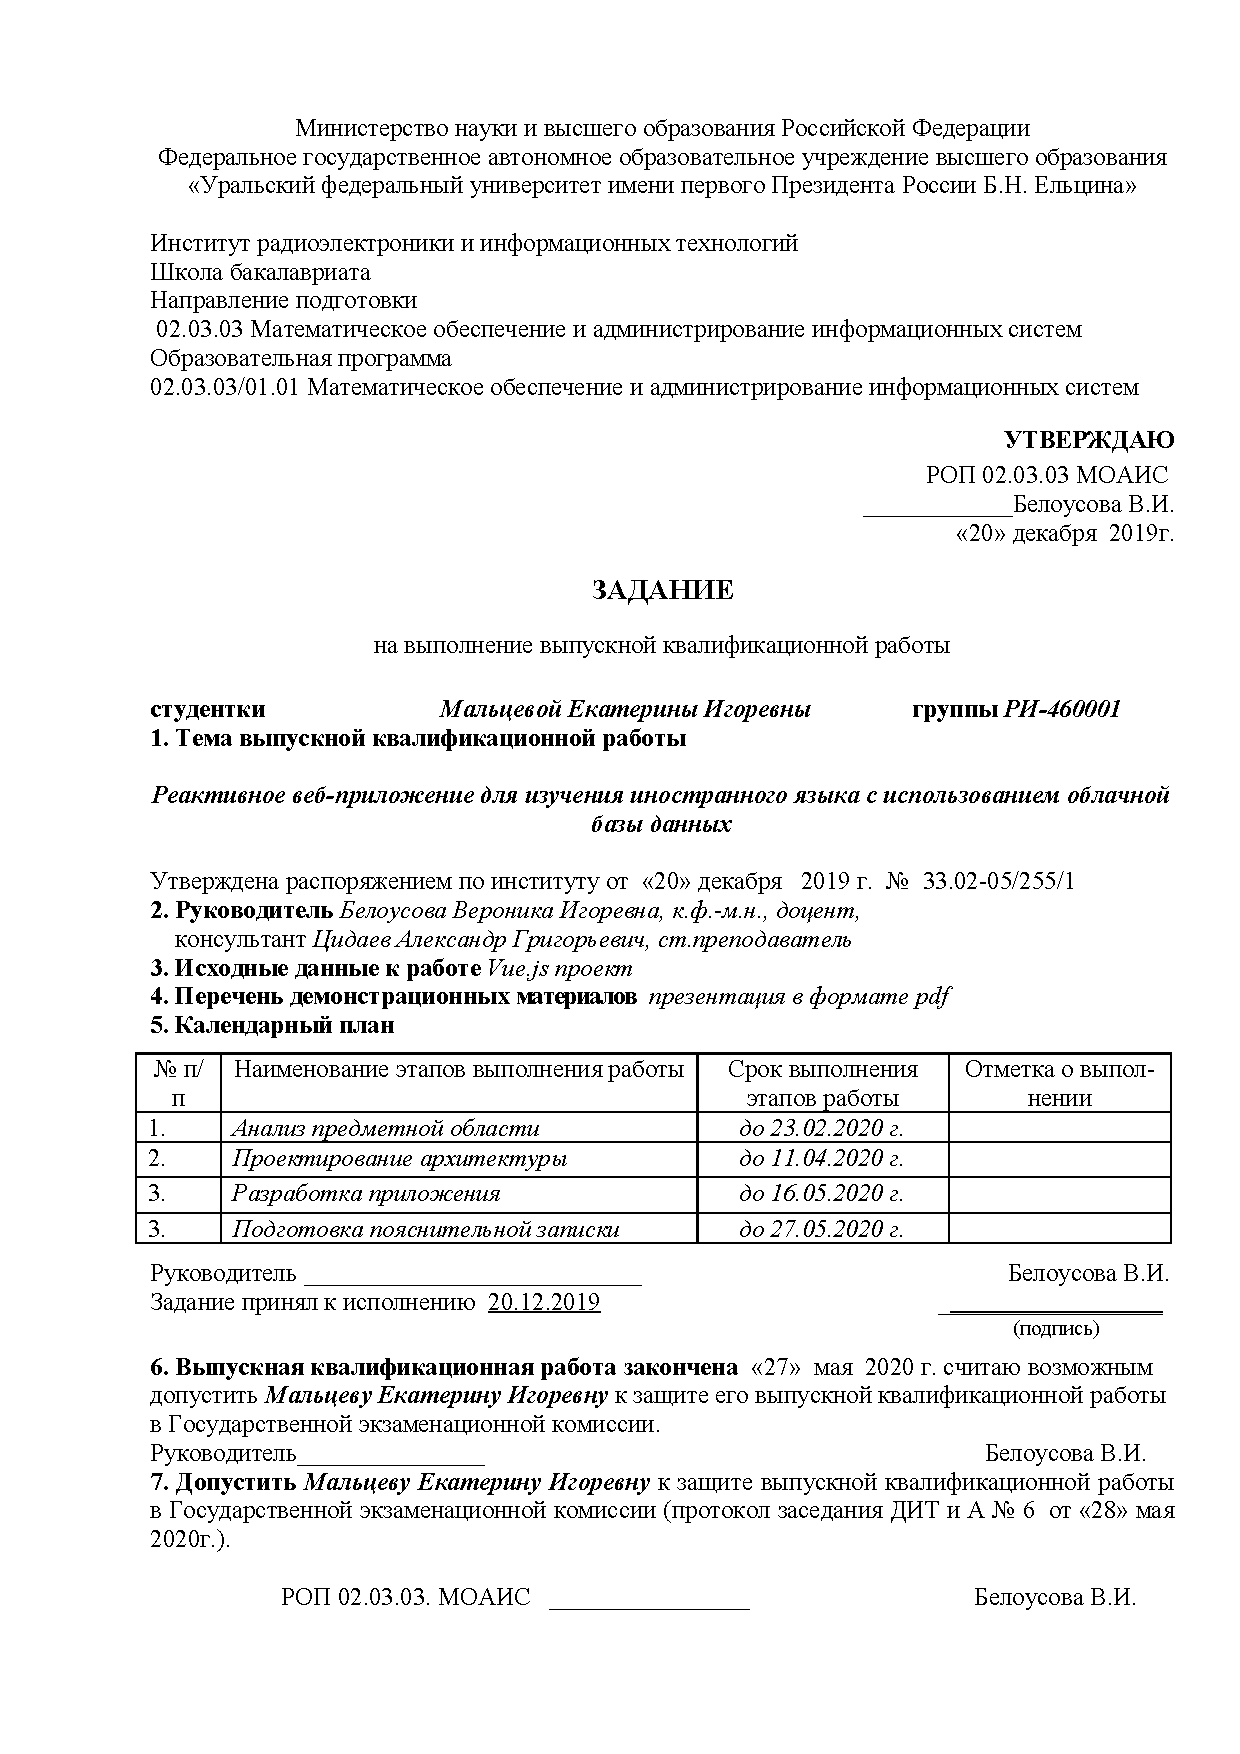
\includegraphics{task.pdf}
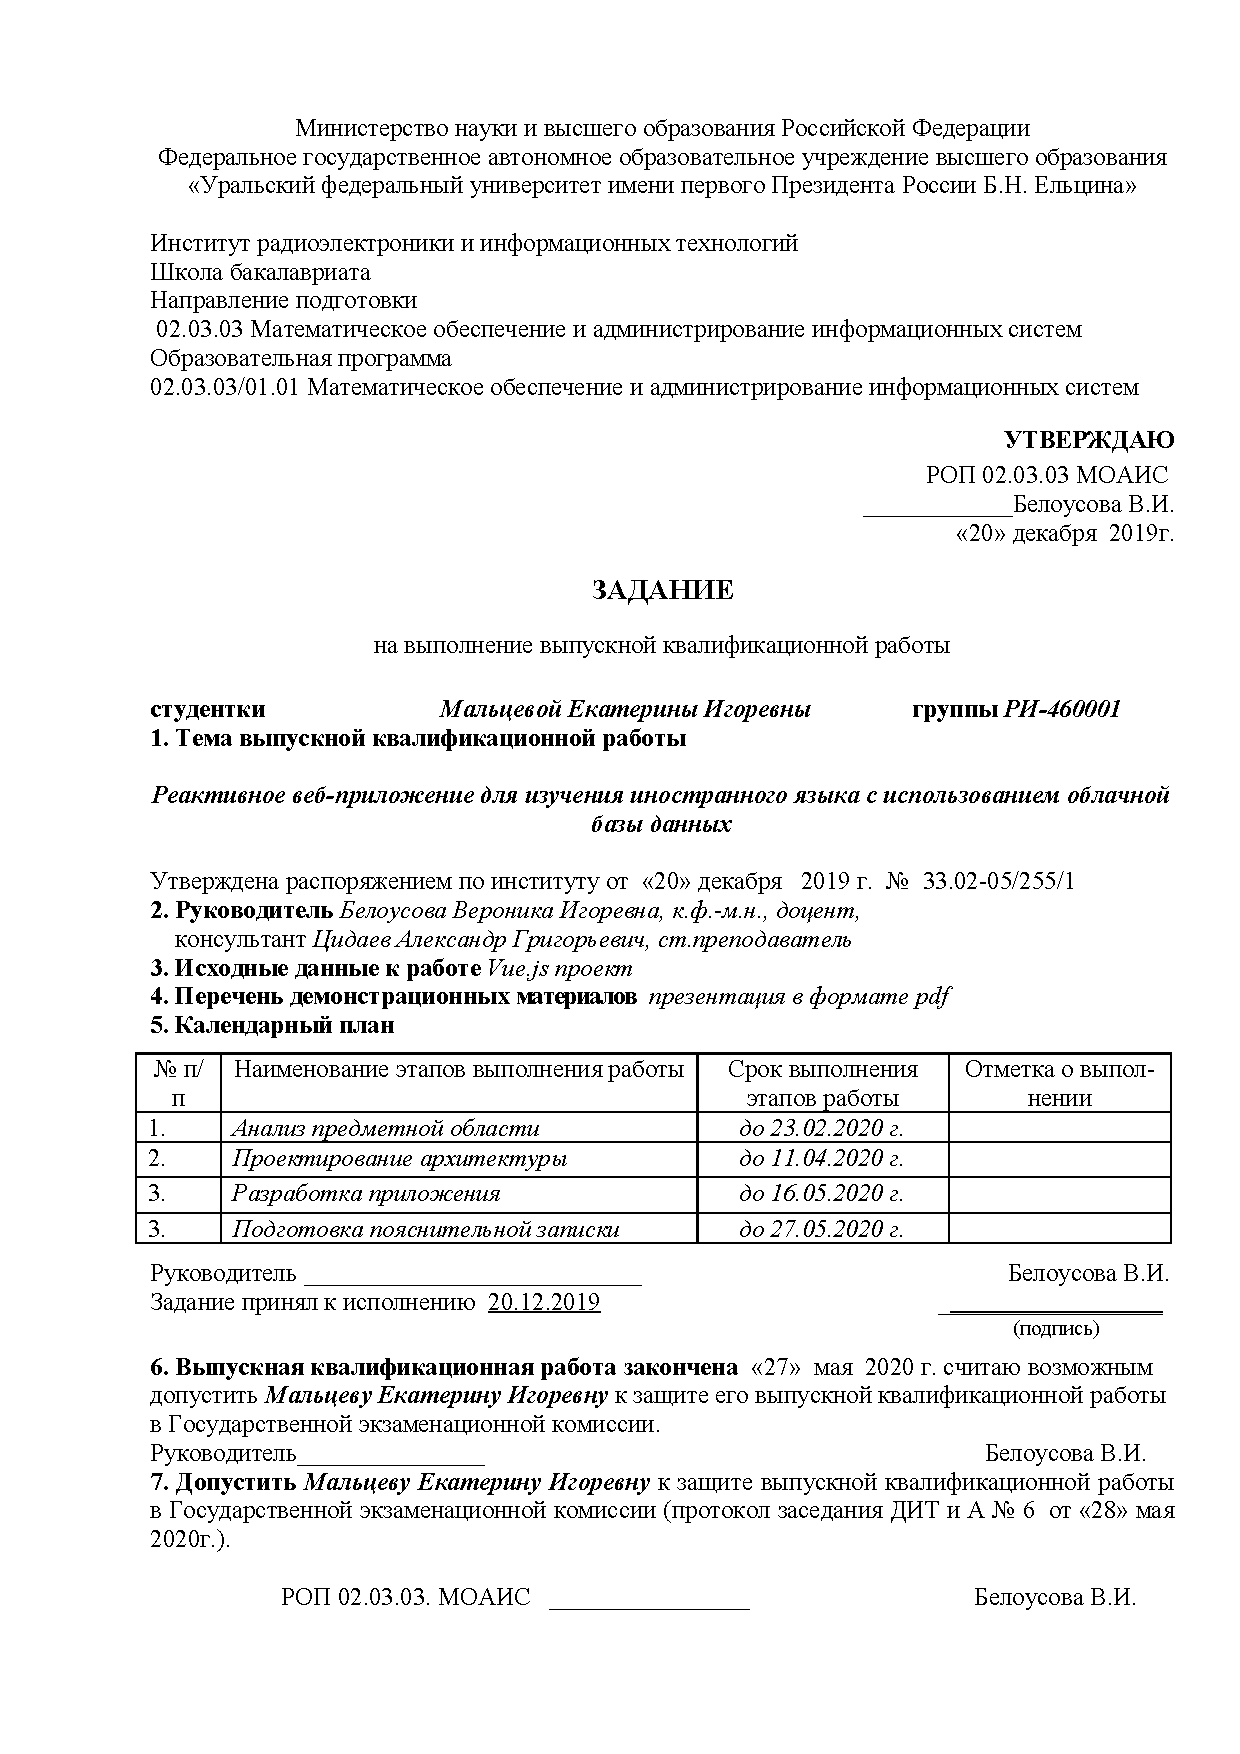
\includepdf[pages=-]{task.pdf}

\frontmatter % выключает нумерацию ВСЕГО; здесь начинаются ненумерованные главы: реферат, введение, глоссарий, сокращения и прочее.

% Команды \breakingbeforechapters и \nonbreakingbeforechapters
% управляют разрывом страницы перед главами.
% По-умолчанию страница разрывается.

% \nobreakingbeforechapters
% \breakingbeforechapters

% Также можно использовать \Referat, как в оригинале
\begin{abstract}
	
Выпускная квалификационная работа содержит \pageref{LastPage}\,страниц, 30 рисунков, 3 таблицы, 13 листингов, 21 источник.

Цель данной работы~--- создание реактивного веб-приложения для изучения иностранного языка.

Результатом данной работы является реактивное веб-приложение на прогрессивном фреймворке Vue.js. Приложение реализует изучение иностранного языка с помощью параллельного чтения и метода интервальных повторений. Реактивность данных обеспечивает интерактивное поведение приложения в ответ на пользовательские действия и положительно влияет на опыт пользователя.

Ключевые слова: компьютерное обучение иностранным языкам, реактивное программирование, облачная инфраструктура, веб-сервис.
\end{abstract}

%%% Local Variables: 
%%% mode: latex
%%% TeX-master: "rpz"
%%% End: 

\pagestyle{plain}

\tableofcontents

%\Defines % Необходимые определения. Вряд ли понадобться
\begin{description}
\item[Распределённый] Слово, которое нельзя употреблять. Но надо протестировать длинные строки в глоссарии.
\end{description}

%%% Local Variables:
%%% mode: latex
%%% TeX-master: "rpz"
%%% End:

\Abbreviations %% Список обозначений и сокращений в тексте
\begin{description}
%\item[SQL] Structured Query Language, <<язык структурированных запросов>>. %Применяется в реляционной модели для управления данными.
\item[NoSQL] Not only Structured Query Language, <<не только SQL>>. Подход, основанный на нереляционной модели базы данных.
\item[API] Application Programming Interface, <<программный интерфейс приложения>>. Посредник между теми или иными сервисами для обеспечения доступа и обмена данными.
\item[HTML] HyperText Markup Language, <<язык гипертекстовой разметки>>. Описывает разметку и применяется для структурирования и представления содержимого веб-страницы.
\item[CSS] Cascading Style Sheets, <<каскадные таблицы стилей>>. Используется для стилизации и общего оформления внешнего вида веб-страницы.
\item[DOM] Document Object Model, <<объектная модель документа>>. Программный интерфейс, который выстраивает иерархическую структуру HTML-документов.
\item[JSON] JavaScript Object Notation, <<текстовый формат обмена данными, основанный на JavaScript>>. Описывает структуру и организацию данных и предоставляет возможность их хранения и передачи.
%\item[MVVM] Model~--- View~--- ViewModel, <<модель~--- представление~--- модель представления>>. Шаблон проектрирования архитектуры приложений, позволяющий создавать приложения, которые мгновенно реагируют на действия пользователя.
\item[NPM] Node Package Manager, <<менеджер пакетов>>. Инструмент для управления программными JavaScript-пакетами, который позволяет производить их установку одной командой.
\end{description}

%%% Local Variables:
%%% mode: latex
%%% TeX-master: "rpz"
%%% End:

\Introduction

\textbf{Актуальность темы.} Компьютерное обучение языкам охватывает широкий спектр приложений и подходов к информационно-коммуникационным технологиям для преподавания и изучения иностранных языков, начиная от традиционных методов обучения, которые зародились в 1960-х и 1970-х годах, и заканчивая более современными подходами с использованием виртуальной учебной среды и дистанционного обучения с помощью Интернета. На сегодняшний день компьютерное обучение иностранным языкам является одним из бурно развивающихся направлений.

Современные методы обучения требуют активного использования компьютерных технологий, которые позволяют усовершенствовать процесс обучения не только преподавателям, но и обучающимся. Нынешняя концепция компьютерного обучения по большей части направлена на самостоятельную работу учащихся: материалы разработаны таким образом, что сочетают в себе различные интерактивные элементы и индивидуальное обучение, что способствует развитию умений и навыков, необходимых учащимся в процессе обучения и самообразования. Однако эффективность данного типа обучения достигается в совокупности с традиционными методами и помогает учителям облегчить процесс обучения языку: к примеру, было изучено влияние использования одной из наиболее популярных онлайн-платформ по изучению иностранных языков~--- Duolingo, внедрив ее в класс студентов, изучающих испанский. Как показывают результаты данного исследования, те студенты, которые на регулярной основе выполняли задания в Duolingo, демонстрировали лучшие результаты на тестах по сравнению с теми студентами, которые не выполняли этих упражнений \cite{sushant}.

\textbf{Объектом исследования} выступают обучающие методы и интерактивные подходы, используемые в современных онлайн-платформах для обучения иностранному языку.

\textbf{Предметом исследования} является моделирование алгоритмов работы обучающих методов для их последующего внедрения в разрабатываемое веб-приложение.

\textbf{Целью исследования} является разработка реактивного веб-приложения для изучения иностранного языка. Под \textit{реактивностью} подразумевается способность приложения отслеживать изменения в своем состоянии, распространять сведения об этих изменениях другим компонентам и вовремя отрисовывать представление данных, а также своевременно реагировать на действия пользователя, что играет немаловажную роль для достижения интерактивности.

Для достижения поставленной цели были сформулированы следующие \textbf{задачи}:

\begin{itemize}
	\item провести анализ наиболее эффективных для обучения педагогических технологий и смоделировать алгоритмы их работы;
	\item изучить документации к инструментам разработки;
	\item осуществить проектирование и разработку приложения.
\end{itemize}

\textbf{Средствами разработки} в данной работе выступают: язык для описания структурной разметки HTML, язык для стилизации элементов CSS, язык программирования JavaScript, веб-фреймворк Vue.js, а также JavaScript-библиотеки с открытым исходным кодом: Axios, Vue Material, Vuelidate, Vuex и Vue Router. В роли серверной составляющей для организации обмена и хранения данных служит облачная нереляционная база данных Cloud Firestore, входящая в состав сервисов Firebase от компании Google.

%%% Local Variables:
%%% mode: latex
%%% TeX-master: t
%%% End:

\mainmatter % это включает нумерацию глав и секций в документе ниже

\chapter{Анализ предметной области}
\label{cha:analysis}
\section{Компьютерное обучение иностранным языкам}

Для решения одной из поставленных задач необходимо определить обучающие методы, благодаря которым пользователь сможет эффективно усваивать знания. Наиболее часто в подобных приложениях можно встретить параллельные тексты и метод интервальных повторений, который чаще всего используется совместно с системой флэш-карточек.

\subsection{Параллельное чтение}

Параллельные тексты, вероятно, являются одним из самых древних методов обучения иностранным языкам. Данный метод заключается в представлении текста таким образом, что повествование идет сразу на двух языках: как правило, на одном обороте представлен исходный текст на изучаемом языке, а на другом~--- переведенный текст на родном языке.

Главное достоинство параллельного чтения~--- развитие <<чувства языка>>: анализируя и сравнивая два текста на разных языках, пользователь начинает лучше понимать структуру предложения, принципы его построения и те или иные языковые особенности.

Сложность в использовании этого метода состоит в том, что пользователю необходимо знать базовую грамматику и правила чтения. Кроме того, немаловажную роль играет качество перевода. Однако стоит отметить, что длительное использование параллельного чтения приводит к постепенному привыканию к различным лексическим и грамматическим конструкциям, что делает данный метод очень интересным и перспективным; также он отлично подходит для пополнения словарного запаса \cite{shepherd}.

\subsection{Метод интервальных повторений}

История появления данного метода началась в конце XIX века, когда немецкий психолог Герман Эббингауз построил «кривую забывания», отражающую то, как долго хранится в памяти однажды запомненная информация. Свои результаты он нанес на график и получил эту «кривую», показанную на рис.~\ref{fig:curve} (картинка взята отсюда \cite{picture}).

\begin{figure}
  \centering
  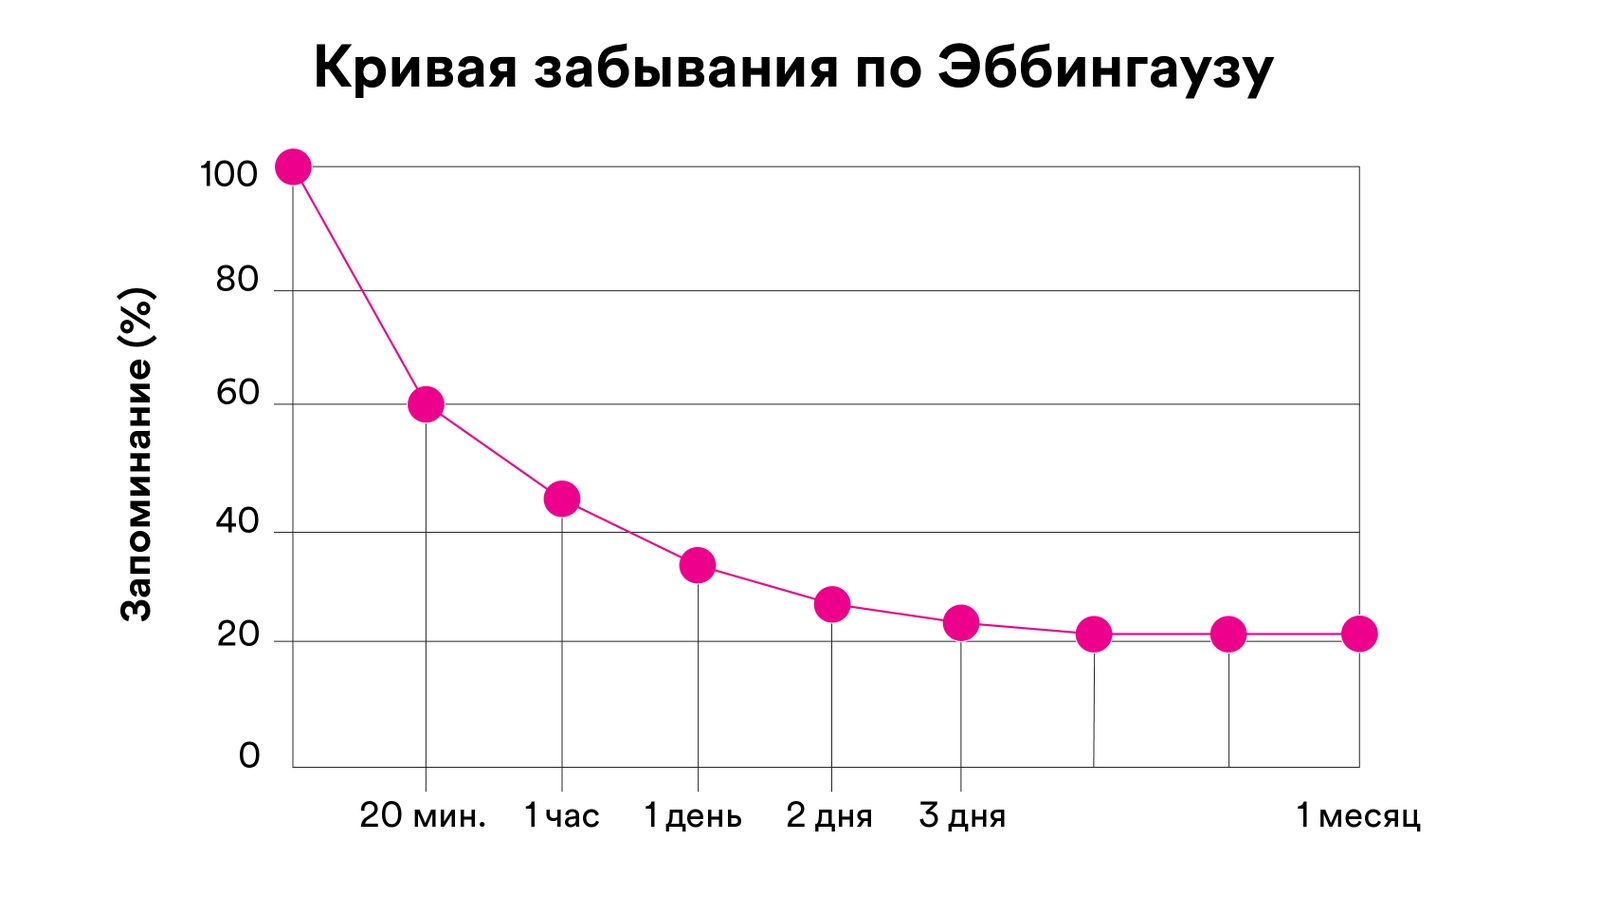
\includegraphics[width=\textwidth]{figures/curve}
  \caption{Кривая забывания}
  \label{fig:curve}
\end{figure}

Согласно его труду, если не пытаться осмысленно повторять однажды заученную информацию, то уже в течение первого часа забывается около 55\% всей информации; к концу дня это число становится равным около 36\%; далее процесс забывания идет медленно, и через неделю, равно как и через месяц, в памяти остается около 20\% от общего числа первоначально выученной информации \cite{ebbinghaus}.

В свою публикацию Эббингауз также включил уравнение аппроксимации этой кривой (\ref{F:F1}), где \textit{k} и \textit{c} — константы, полученные при определенных вычислениях (\textit{k} = 1.84, \textit{c} = 1.25), значение \textit{b} отражает «удержание» информации в процентах, тогда как \textit{t} равно времени в минутах.

\begin{equation}
b = 100 \times \frac{k}{{(\log_{10} t)}^c + k}
\label{F:F1}
\end{equation}

Впоследствии Эббингауз открыл \textit{закон накопления и распределения повторений}, окончательно сформулированный в 1895 году немецким психологом Адольфом Йостом. Согласно этому закону, при фиксированном количестве повторений распределенные во времени повторения более эффективны, чем одновременные.

Затем эта идея получила развитие в 1932 году, когда британский философ Алек Мейс разработал метод интервальных повторений \cite{mace}. Суть остается такой же: если осмысленно воспроизводить заученный материал через определенные, постоянно возрастающие интервалы времени, можно добиться более эффективных результатов и удержать выученную информацию на более длительные сроки.

В 1939 году было проведено исследование, в котором принимали участие более 3600 студентов, в ходе которого была доказана эффективность данного метода \cite{spitzer}. Несмотря на то, что эта техника подойдет для запоминания любой информации, наибольшее распространение она получила именно при изучении иностранных языков.

Как уже было упомянуто ранее, интервальные повторения часто используют совместно с системой флэш-карточек, также известной как система Лейтнера. Это простая реализация метода интервальных повторений, предложенная немецким журналистом и популяризатором науки Себастьяном Лейтнером в 1970-х годах \cite{leitner}. Она наглядно показана на рис.~\ref{fig:leitner}.

\begin{figure}
	\centering
	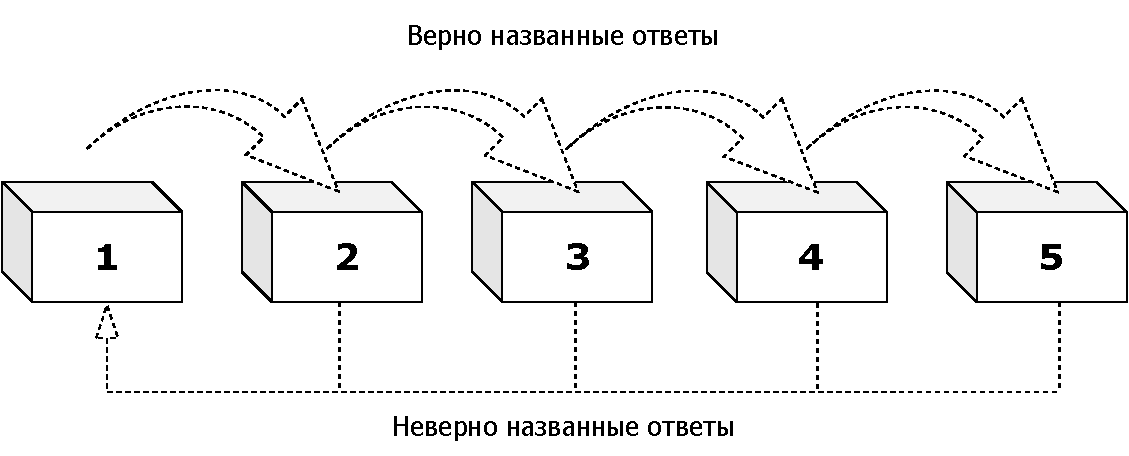
\includegraphics[keepaspectratio, scale=0.8]{figures/leitner}
	\caption{Система Лейтнера}
	\label{fig:leitner}
\end{figure}

Работает эта система следующим образом: в самом начале любое слово, представленное в виде карточки, всегда находится в первой коробке; если пользователь вспоминает его значение и отвечает правильно, то карточка перекладывается в следующую коробку, если отвечает неправильно — карточка возвращается назад в первую коробку, независимо от того, в какой коробке находилась на последней итерации. И каждое следующее слово повторяется через увеличивающийся интервал времени. Например, можно увеличивать время следующего повторения в три раза: в таком случае первое повторение наступит через день, второе~--- через 3 дня, третье~--- через 9 дней, четвертое~--- через 27 и т.~д.

\section{Обзор существующих приложений, предназначенных для обучения иностранным языкам}

В настоящее время существует достаточно обширное количество программных платформ для изучения иностранных языков. Стоит признать, что подавляющее большинство таких приложений преобладает на мобильном рынке, и чаще всего такие приложения являются либо платными, либо условно-бесплатными, причем условно-бесплатные решения сильно ограничены по своему функционалу и контентному содержимому. По этой причине мобильный сегмент рассматриваться не будет.

В рамках проведенного обзора были рассмотрены следующие наиболее популярные приложения, которые помогают в освоении иностранного языка:

\begin{itemize}
\item \textbf{Anki}~--- программа, предназначенная для облегчения запоминания слов, выражений и любой другой информации с помощью метода интервальных повторений;
\item \textbf{Duolingo}~--- бесплатный веб-сервис, который привлекает своим простым и понятным интерфейсом и игровым подходом к изучению иностранных языков.
\end{itemize}

\subsection{Anki}

Данная программа распространяется под свободной лицензией и доступна для использования на различных операционных системах: Microsoft Windows, macOS, Linux и FreeBSD. Существует веб-версия этого приложения с поддержкой хостинга колод и наличием разнообразных плагинов. Также авторами поддерживается мобильное приложение для iOS с закрытым исходным кодом.

Anki предоставляет пользователю следующий ряд интересных действий и возможностей:

\begin{itemize}
	\item создавать собственные карточки и настраивать их внешний вид различными способами: с помощью гипертекстовой разметки со стилями или продвинутыми средствами \LaTeX{}, а также оснащать их изображениями, звуками и мультимедийными файлами;
	\item настраивать алгоритмы обучения под собственные нужды;
	\item синхронизировать карточки между несколькими устройствами;
	\item просматривать подробную статистику в виде цифр и графиков.
\end{itemize}

Anki использует алгоритм, основанный на методе интервального повторения. Интерфейс десктопного приложения Anki представлен на рис.~\ref{fig:anki}. При нажатии кнопки <<Показать ответ>> необходимо указать то, насколько легко пользователю далось данное слово: <<не помню>>, <<в самый раз>>, <<очень легко>>. На основании статистики полученных ответов Anki определяет, какую карточку и когда нужно показывать для последующего повторения.

\begin{figure}[h]
	\centering
	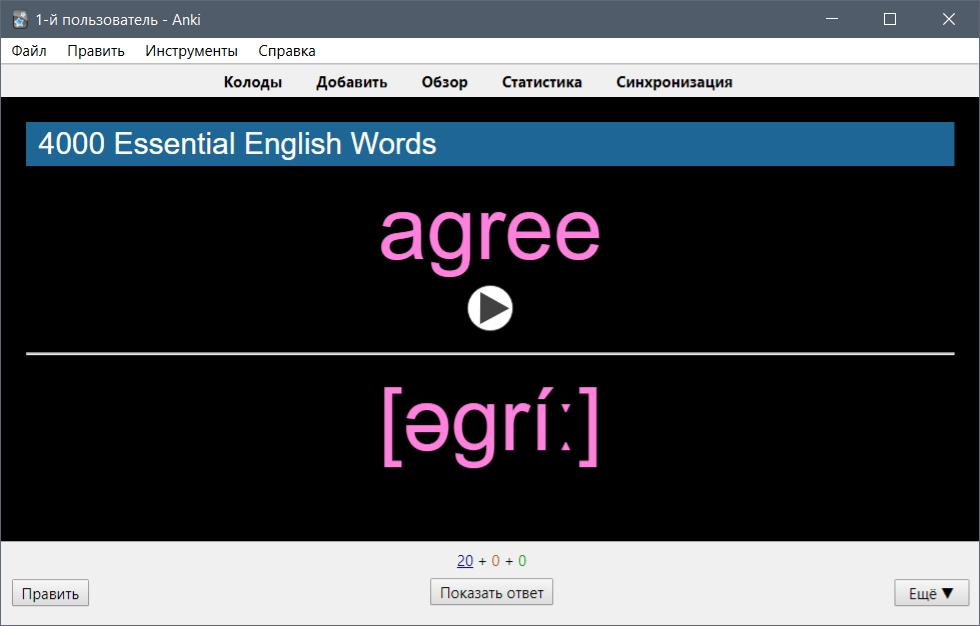
\includegraphics[keepaspectratio, scale=0.7]{figures/anki}
	\caption{Программный интерфейс десктопной версии Anki}
	\label{fig:anki}
\end{figure}

Можно практиковать как свои колоды карт, так и готовые колоды из Интернета. Более продвинутые колоды оснащены возможностью озвучивания слов и прочтения их транскрипций.

\subsection{Duolingo}

Duolingo является наиболее популярным веб-сервисом в международном сегменте. Платформа поддерживает обширный перечень языков и предлагает многочисленные вариации обучения: благодаря игровому дереву происходит продвижение по урокам, а в словарном разделе пользователи могут практиковать новые слова. Фрагмент игрового дерева представлен на рис.~\ref{fig:duo}.

\begin{figure}[h]
	\centering
	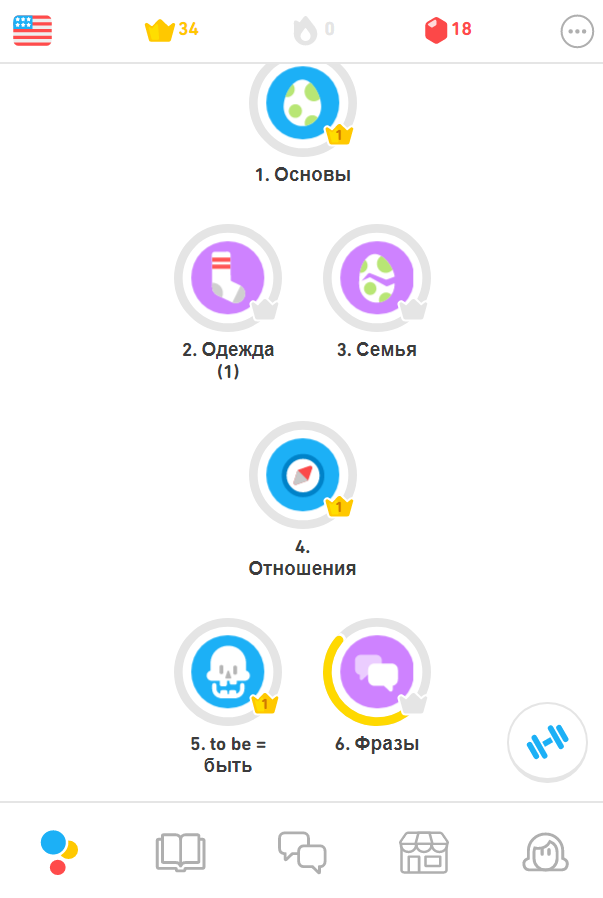
\includegraphics[width=0.6\textwidth, keepaspectratio]{figures/duo}
	\caption{Игровое дерево в Duolingo}
	\label{fig:duo}
\end{figure}

Для привлечения пользователей платформа имитирует структуру видеоигр: например, за счет системы вознаграждений пользователи могут получить внутреигровую валюту, которую можно потратить на бонусные уровни. Также существуют значки, которые представляют собой достижения и указывают на уровень квалификации пользователя.

В Duolingo также существуют системы форумов и т.~н. <<списки лидеров>>, которые позволяют повысить конкурентоспособность и отношения между пользователями, добавив учебному процессу больше веселья, что позволяет повысить мотивацию к обучению.

Главной особенностью Duolingo являются индивидуальные уроки: система запоминает и учитывает трудности, которые возникли у пользователя во время изучения языка, и использует эти данные для машинного обучения. Кроме того, по мере прохождения уроков пользователи параллельно помогают переводить сайты и различные документы.

Данная платформа доступна как в виде веб-приложения, так и в форме приложения под мобильные устройства на iOS и Android, однако далеко не все функции и возможности веб-приложения доступны в мобильной версии: к примеру, в ней отсутствует грамматическая справка, в которой приводится краткая сводка основных правил перед прохождением урока; также в мобильной версии нет возможности выбрать тренировку на время и общаться с другими пользователями на форуме.

\section{Вывод}

В данном разделе был проведен анализ предметной области, на основе которого были сделаны следующие выводы и наблюдения:

\begin{itemize}
	\item рассмотренные методики обучения имеют доказанную эффективность на основе ряда исследований и могут быть использованы для разрабатываемого приложения;
	\item геймификация процесса обучения и возможность пользовательского взаимодействия друг с другом~--- неотъемлемые черты подобных приложений для поддержания мотивации к обучению;
	\item возможным решением задачи обеспечения взаимодействия пользователя с разрабатываемым приложением является создание адаптивного веб-интерфейса, доступного под любые устройства через веб-браузер;
	\item одностраничные приложения выступают наиболее удачным решением для достижения интерактивного взаимодействия пользователя с веб-интерфейсом: мгновенная отрисовка данных и переключение между состояниями приложения благоприятно влияют на пользовательский опыт.
\end{itemize}

Проведенный обзор также показал распространенность использования веб-приложений для компьютерного обучения, что еще раз подчеркивает актуальность данной работы. Кроме того, ни одно из рассмотренных популярных приложений не сочетает в себе совместное использование метода параллельного чтения и системы интервальных повторений, что делает данную работу уникальной.

Таким образом, с учетом сделанных выводов становится возможным создание веб-приложения, в котором будут учтены наблюдения, подмеченные в данном разделе.

%%% Local Variables:
%%% mode: latex
%%% TeX-master: "rpz"
%%% End:

\chapter{Обзор средств разработки и проектирование приложения}
\label{cha:design}

\section{Использованное оборудование}
В таблице \ref{tab:tab1} приведены краткие технические характеристики оборудования, на котором производилась разработка приложения.

\begin{table}
	\centering
	\begin{tabular}{ |l|l|c|c| } 
		\hline
		Процессор & Intel(R) Core(TM) i5-4200H \\
		\hline
		Базовая тактовая частота процессора & 2.8 GHz \\
		\hline
		Количество ядер процессора & 2 \\
		\hline
		Объем ОЗУ & 8 Гб \\
		\hline
		Операционная система & Windows 10 Pro \\ 
		\hline
	\end{tabular}
	\caption{Технические характеристики оборудования}
	\label{tab:tab1}
\end{table}

\section{Инструменты разработки}

В качестве среды разработки был выбран текстовый редактор Visual Studio Code. Данный выбор обусловлен в первую очередь легковесностью по сравнению с полноценными интегрированными средами разработки (WebStorm, Visual Studio и~др.) и богатым разнообразием дополнительных расширений. Кроме того, данный редактор является кросплатформенным и распространяется бесплатно, а также имеет интеграцию с системой контроля версий Git.

\subsection{Клиентская часть приложения}

Появление JavaScript в 1995 году сделало возможным применение современных веб-приложений~--- приложений, с которыми можно взаимодействовать без перезагрузки страницы при каждом действии пользователя. Изначально он создавался для придания интерактивности веб-страницам, но, как показывает картина, на сегодняшний день JavaScript является самым распространенным решением для разработки приложений на стороне клиента и одним из самых популярных~--- на серверной стороне.

Примечательно то, что JavaScript~--- это не только язык, но и целая инфраструктура, состоящая из огромного количества фреймворков и библиотек. Их разнообразие столь колоссально, что выделить лучший становится невозможно, поэтому выбор фреймворка для того или иного решения остается личным предпочтением разработчика или компании. А вручную описывать манипуляции с иерархической структурой гипертекстовой разметки на <<ванильном>> JavaScript является довольно ресурсоемкой задачей даже для небольшого проекта. Хотя бы по этой причине в современном мире есть огромная необходимость во фреймворках.

Опираясь на выводы, сделанные в разделе 1, было принято решение о реализации клиентской части в виде одностраничного приложения с использованием фреймворка. На момент написания данной работы наиболее популярными фреймворками для создания одностраничных приложений являются Angular, React и Vue.js.

В данном проекте для обеспечения работы клиентской части приложения был выбран фреймворк \textbf{Vue.js} \cite{vuejs}. Данный выбор обусловлен наличием у автора этой работы опыта разработки на выбранном фреймворке. Стоит выделить основные преимущества, которыми он обладает:

\begin{itemize}
	\item \textbf{Реактивность.} Состояние интерфейса приложения автоматически реагирует на изменение данных;
	\item \textbf{Легковесность.} Минимизированный и сжатый файл Vue.js занимает примерно 24 Кб, что довольно скромно для прогрессивного фреймворка;
	\item \textbf{Производительность.} Vue.js использует Virtual DOM: все операции выполняются с не привязанным к браузеру представлением DOM, после чего внесенные изменения копируются на саму страницу, что и обеспечивает высокую производительность \cite{stefankrause};
	\item \textbf{Интеграция.} Vue.js легко адаптировать и внедрить в уже существующий проект, не оказывая при этом негативного влияния на всю систему;
	\item \textbf{Масштабируемость.} Vue.js позволяет создавать крупные шаблоны и переиспользовать их, что значительно сокращает затраты на разработку;
	\item \textbf{Низкий порог вхождения.} Любое приложение на Vue.js пишется с помощью знакомых любому веб-разработчику технологий: HTML для разметки страницы, CSS для стилизации элементов и JavaScript для обеспечения интерактивного взаимодействия с конечным пользователем.
\end{itemize}

Также на клиентской части приложения используется официальный роутер Vue Router \cite{vuerouter}, отвечающий за маршрутизацию одностраничного приложения, и библиотека управления состоянием Vuex \cite{vuex}. В качестве вспомогательных библиотек разрабатываемого приложения выступают такие библиотеки, как Axios \cite{axios}, Vuelidate \cite{vuelidate} и Vue Material \cite{vuematerial}.

\subsection{Серверная часть приложения}

При создании веб-приложения основную роль занимает разработка серверной части. Есть два варианта: развернуть сервер самостоятельно или использовать уже готовое решение. Для поставленных целей вполне подойдет \textbf{Firebase}~--- продукт компании Google для быстрого создания мобильных и веб-приложений \cite{firebase}.

Firebase включает в себя множество полезных сервисов, но основным является облачная система управления базами данных класса NoSQL, позволяющая хранить и синхронизировать данные между несколькими пользователями. Firebase еще хорош тем, что автоматически масштабируется и после внедрения в проект позволяет сразу же приступать к разработке. Для полноты картины ниже будут перечислены все сервисы Firebase, использованные в данной работе:

\begin{itemize}
	\item \textbf{Firebase Auth.} Данный сервис позволяет аутентифицировать пользователей. Также доступна система управления пользователями, в соответствии с которой можно включить аутентификацию с помощью электронной почты и пароля;
	\item \textbf{Cloud Firestore.} Гибкая, масштабируемая облачная база данных, которая позволяет хранить данные и легко получать к ним доступ, а также следить за изменениями в режиме реального времени;
	\item \textbf{Firebase Storage.} Хранилище обеспечивает доступ к файлам пользователей. Можно использовать этот сервис для хранения пользовательского контента, например, различных медиафайлов;
	\item \textbf{Firebase Hosting.} Этот сервис поддерживает размещение статических файлов (HTML, CSS, JavaScript и т.~д.) и позволяет произвести быструю развертку приложения одной командой.
\end{itemize}

\section{Концепт приложения}

Исходя из проведенного анализа в разделе 1 следует определить основной процесс, благодаря которому пользователь сможет усваивать знания и взаимодействовать с приложением в целом. Этот процесс в разрабатываемом приложении выглядит следующим образом:

\begin{itemize}
	\item чтобы имплементировать метод параллельного чтения, в разрабатываемом приложении необходим модуль, отвечающий за книги и их части: посредством чтения книг с параллельным переводом пользователь сможет добавлять не знакомые ему слова в свой личный словарь для изучения;
	\item для имплементации метода интервальных повторений в разрабатываемом приложении необходим модуль, отвечающий за пользовательские данные: непосредственно при чтении книг все добавленные слова будут помещены именно в этот модуль, в котором также будет определена логика запоминания слов;
	\item чтобы пользователи могли делиться опытом изучения иностранного языка и задавать вопросы друг другу, в разрабатываемом приложении необходимы модули, отвечающие за статьи и форум, которые помогут повысить мотивацию к обучению.
\end{itemize}

\section{Задачи и требования}

С учетом выбранных инструментов разработки и общей идеи приложения, обозначенных в двух предыдущих подразделах, следует определить основной функционал, которым должно обладать разработанное приложение.

Веб-приложение должно обеспечивать аутентификацию пользователей: получение введенных из формы данных и сохранение входа после перезагрузки страницы, а также обработка ошибок и защита от несанкционированного входа.

Также в разрабатываемом приложении должен быть компонент, отвечающий за функциональность личного кабинета:

\begin{enumerate}
	\item возможность изменять личные данные пользователя: имя, электронную почту, пароль и изображение профиля;
	\item просмотр персональной информации, связанной с обучением: набор слов для изучения, представленный в виде таблицы, а также все книги, добавленные пользователем.
\end{enumerate}

Помимо этого в веб-приложении должна быть разработана система форумов, состоящая из разделов, каждый из которых нацелен на определенную тематику: 

\begin{enumerate}
	\item возможность фильтрации тредов по трем типам: треды пользователя, решенные и нерешенные треды;
	\item возможность создавать, редактировать и удалять треды, а также оставлять комментарии к ним (комментарии также можно удалять);
	\item автор треда может помечать один из комментариев к треду как решение своей проблемы.
\end{enumerate}

Плюс ко всему разрабатываемое приложение должно иметь компонент, отвечающий за систему пользовательских статей:

\begin{enumerate}
	\item возможность фильтрации статей по трем типам: статьи пользователя, статьи людей, на которых пользователь подписан, и понравивишеся статьи;
	\item возможность создавать, редактировать и удалять статьи, а также оставлять комментарии к ним (комментарии также можно удалять).
\end{enumerate}

Вдобавок в приложении необходим компонент, отвечающий за просмотр списка книг и возможность поиска и фильтрации по уровню подготовки, а также компонент для просмотра подробной информации о каждой отдельно взятой книге и ее частях с возможностью ее добавления в личную библиотеку.

Чтение частей книги должно осуществляться с возможностью переводить отдельные слова или целые предложения и добавлять их в личный словарь для изучения.

Также в веб-приложении необходим динамический тренажер для запоминания добавленных пользователем слов с возможностью озвучивания слова.

Кроме всего прочего для разрабатываемого приложения необходимо обеспечить безопасность данных посредством настройки правил для базы данных и защиты маршрутов.

И, наконец, разрабатываемое приложение должно быть снабжено адаптивным пользовательским интерфейсом.


\section{Архитектура приложения}

С учетом выбранных и обоснованных инструментов разработки, обозначенных в данном разделе, была также определена архитектура клиентской и серверной частей веб-приложения. Она изображена на рис.~\ref{fig:arch} и представляет из себя прямое взаимодействие веб-приложения на Vue.js с сервисами Firebase через его API. В разделе 3 описано, как именно и с помощью каких инструментов осуществляется данное взаимодействие.

\clearpage

\begin{figure}[h]
	\centering
	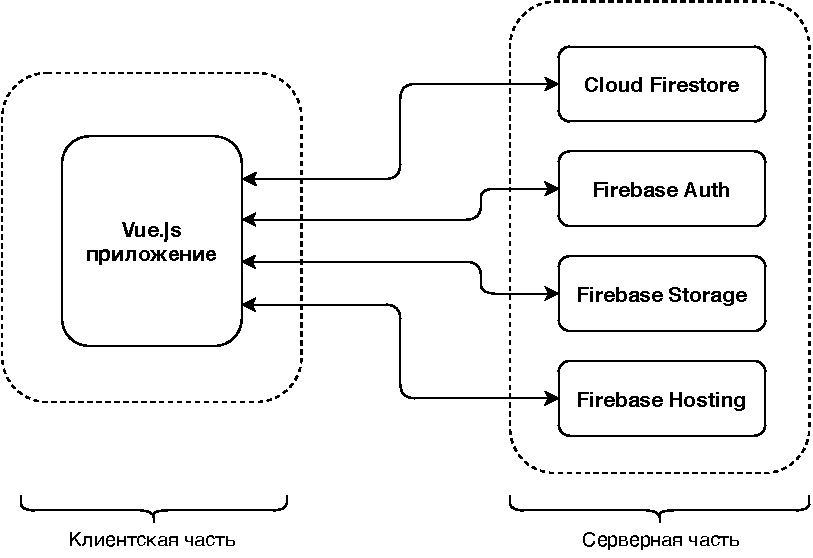
\includegraphics[width=\textwidth, keepaspectratio]{figures/arch}
	\caption{Архитектура приложения}
	\label{fig:arch}
\end{figure}

\section{Вывод}

Таким образом, опираясь на выводы из предыдущего раздела, в рамках данного раздела были решены следующие задачи:

\begin{itemize}
	\item проведен краткий обзор используемого оборудования и обоснованы инструменты разработки, т.~е. были выбраны основные средства для реализации разрабатываемого приложения;
	\item сформулированы задачи и требования, поставленные к разрабатываемому приложению, а также описан его базовый функционал;
	\item на основании поставленных требований с учетом используемых инструментов разработки была определена архитектура проекта.
\end{itemize}

%%% Local Variables:
%%% mode: latex
%%% TeX-master: "rpz"
%%% End:

\chapter{Разработка приложения}
\label{cha:impl}

\section{Подготовка рабочего окружения}

Такой прогрессивный фреймворк, как Vue.js, очень легко интегрировать в проект: достаточно просто добавить на страницу JavaScript-файл и подключить его тегом \texttt{<script>}. Однако при создании крупных приложений рекомендуется использовать более продвинутые инструменты разработки, такие как пакетный менеджер \textbf{npm} \cite{npm} и компилятор JavaScript-кода \textbf{Babel} \cite{babel}.

\subsection{Менеджер пакетов npm}
Данный пакетный менеджер входит в состав программной платформы Node.js \cite{nodejs}. Главное преимущество npm в том, что его использование упрощает работу с модулями, необходимыми для работоспособности приложения, и производит их установку одной командой.

«Сердцевиной» любого приложения с модулями является файл \texttt{package.json}, который автоматически добавляется в папку с проектом при установке какого-либо пакета. Этот файл содержит в себе всю информацию о разрабатываемом приложении: наименование проекта, его автор, версия и описание, а также различные зависимости, указывающие на названия и версии пакетов, необходимых для работы приложения. В листинге \ref{lst:json} показана часть содержимого этого файла для разрабатываемого приложения.

\subsection{Транспилятор Babel}
\textbf{Babel}~--- это инструмент, который позволяет \textit{транспилировать} код, т.~е. выполнять преобразование современного кода в более ранний стандарт. Проблема заключается в поддержке браузерами различных версий JavaScript: не каждый браузерный движок полностью поддерживает стандарты ES7 и новее \cite{ecma}. По этой причине применение транспилера позволяет разработчикам использовать новейшие возможности языка JavaScript и не терять при этом совместимости со старыми движками браузеров.

\lstinputlisting[
caption=Файл package.json,
label=lst:json]
{listings/package.json}

\section{Клиентская часть приложения}

\subsection{Структура проекта}

Структура проекта в общем виде подробно описана на рис.~\ref{list:struct}. Все ресурсы и исходный код клиентской части веб-приложения находятся в директории \textit{src}.

\begin{figure}
	\dirtree{%
		.1 linguium/.
		.2 node-modules/
		\dotfill
		\begin{minipage}[t]{8cm}
			установленные пакеты npm
		\end{minipage}.
		.2 src/
		\dotfill
		\begin{minipage}[t]{8cm}
			исходные файлы проекта
		\end{minipage}.
		.3 assets/
		\dotfill
		\begin{minipage}[t]{8cm}
			статические ресурсы проекта
		\end{minipage}.
		.3 components/
		\dotfill
		\begin{minipage}[t]{8cm}
			все компоненты проекта
		\end{minipage}.
		.4 auth/
		\dotfill
		\begin{minipage}[t]{8cm}
			компоненты, отвечающие за авторизацию и аутентификацию
		\end{minipage}.
		.4 books/
		\dotfill
		\begin{minipage}[t]{8cm}
			компоненты, отвечающие за книги и их части
		\end{minipage}.
		.4 profile/
		\dotfill
		\begin{minipage}[t]{8cm}
			компоненты, отвечающие за профиль пользователя и его данные
		\end{minipage}.
		.4 ui/
		\dotfill
		\begin{minipage}[t]{8cm}
			компоненты, отвечающие за пользовательский интерфейс
		\end{minipage}.
		.4 ....
		.3 config/
		\dotfill
		\begin{minipage}[t]{8cm}
			конфиги: API яндекса и firebase
		\end{minipage}.
		.3 router/
		\dotfill
		\begin{minipage}[t]{8cm}
			роутер проекта
		\end{minipage}.
		.3 store/
		\dotfill
		\begin{minipage}[t]{8cm}
			папка с модулями хранилища Vuex
		\end{minipage}.
		.3 App.vue
		\dotfill
		\begin{minipage}[t]{8cm}
			корневой компонент проекта
		\end{minipage}.
		.3 main.js
		\dotfill
		\begin{minipage}[t]{8cm}
			точка входа приложения
		\end{minipage}.
		.3 ....
		.2 index.html
		\dotfill
		\begin{minipage}[t]{8cm}
			корневой HTML-шаблон
		\end{minipage}.
		.2 package.json
		\dotfill
		\begin{minipage}[t]{8cm}
			основная информация о проекте и его список зависимостей
		\end{minipage}.
		.2 ....
	} 
	\caption{Структура проекта}
	\label{list:struct}
\end{figure}

\subsection{Глобальное хранилище данных}

\textbf{Vuex}~--- это библиотека для управления состоянием, которая создает глобальное хранилище данных, доступное для всех компонентов приложения, в которых состояние может быть изменено исключительно предсказуемым образом.

Крупные приложения обычно состоят из большого числа компонентов, которые часто подлежат переиспользованию, и обмен данными между ними становится трудно отслеживать. Благодаря хранилищу все состояние приложения может быть представлено в одном месте, что делает приложение более организованным.

Vuex реализует подход к управлению состоянием, основанный на однонаправленном потоке данных. Его простейший вид представлен на рис.~\ref{fig:vuex}.

\begin{figure}
	\centering
	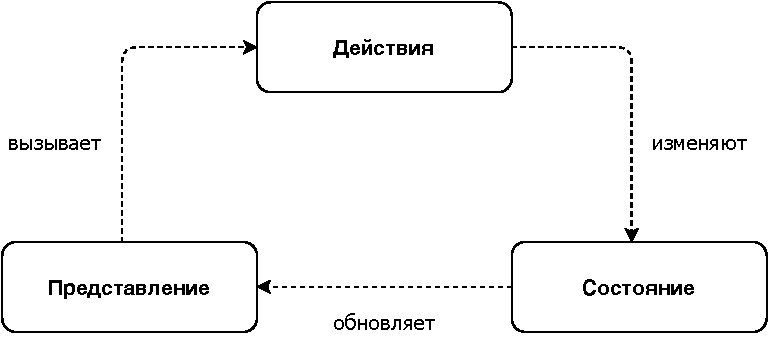
\includegraphics[width=0.9\textwidth, keepaspectratio]{figures/vuex}
	\caption{Однонаправленный поток данных}
	\label{fig:vuex}
\end{figure}

Однако для нескольких компонентов, зависящих от одного и того же состояния, описанный на рис.~\ref{fig:vuex} подход не работает. Данная проблема решается следующим образом: сперва вводится понятие общего состояния всего приложения, которое изменяется с помощью синхронных транзакций~--- \textbf{мутаций} (англ. \textit{mutations}). Мутации в свою очередь выполняются в ответ на асинхронную операцию~--- \textbf{действие} (англ. \textit{action}). И, наконец, действие инициирует мутацию через \textbf{диспетчер} (англ. \textit{dispatcher}).

Обновленная схема организации однонаправленного потока данных с использованием Vuex изображена на рис.~\ref{fig:vuex2}.

\begin{figure}
	\centering
	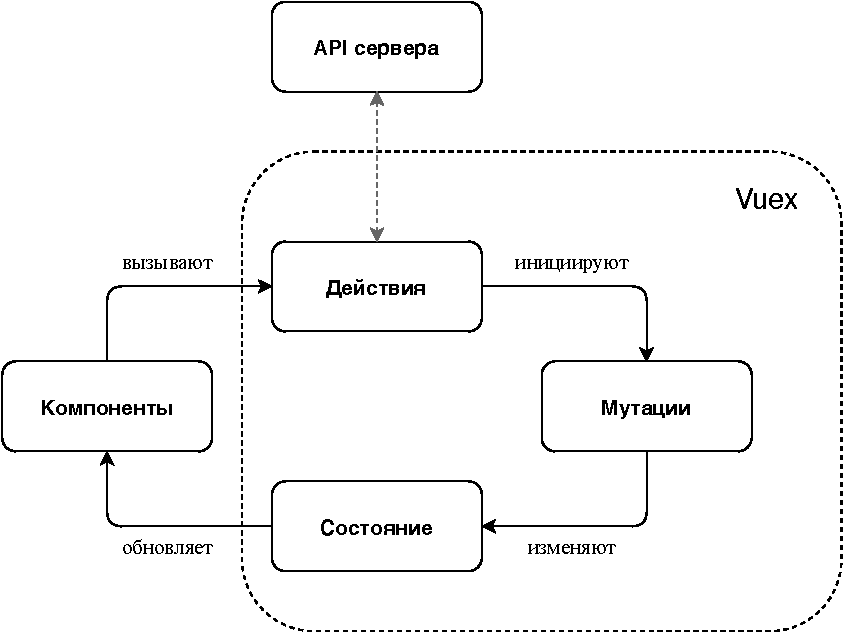
\includegraphics[width=0.95\textwidth, keepaspectratio]{figures/vuex2}
	\caption{Однонаправленный поток данных с Vuex}
	\label{fig:vuex2}
\end{figure}

При данном подходе дерево компонентов становится одним большим <<представлением>>, и любой компонент всегда сможет получить доступ к состоянию приложения или вызывать действие для изменения состояния. Таким образом подчеркивается независимость между представлением и состоянием, а также обеспечивается хорошая структурированность всего приложения и облегчение его отладки.

По умолчанию глобальные данные о состоянии всего приложения хранятся в одном объекте, в результате чего возникают проблемы со структурой данного объекта. По этой причине принято разделять хранилище на \textit{модули}, каждый из которых содержит независимые блоки глобального состояния, в которых есть свои собственные локальные мутации, действия и т.~п. Это также решает возможные проблемы с именованием, т.~к. у каждого модуля будет собственное пространство имен.

Хранилище, используемое в разрабатываемом приложении, было разделено на следующие модули:

\begin{itemize}
	\item информация о всех доступных книгах и их частях (модуль \textit{books});
	\item состояние текущего пользователя и доступные ему операции: авторизация, аутентификация, выход из учетной записи, изменение собственных данных и т. п. (модуль \textit{user});
	\item информация обо всех зарегистрированных учетных записях: имя, электронная почта и аватар каждого пользователя (модуль \textit{users});
	\item все статьи, написанные пользователями, и комментарии к этим статьям: возможность создавать, редактировать и удалять данные (модуль \textit{articles});
	\item система форума, состоящая из пользовательских тредов: функционал тот же, что и в модуле \textit{articles} (модуль \textit{forum});
	\item пользовательские данные: информация о всех прочитанных частях книг (момент времени, в который пользователь последний раз открывал ту или иную часть или же прочитал ее), а также информация о всех пользовательских словах, добавленных в процессе чтения, и все доступные операции над ними (модуль \textit{userdata}).
\end{itemize}

В качестве примера рассмотрим модуль \textit{books}, представленный в листинге \ref{lst:books}. Дадим некоторые пояснения:

\begin{itemize}
	\item в объекте \texttt{state} хранится состояние, содержащее пустой массив под названием books, который вскоре будет заполнен объектами (книгами) с помощью действия \texttt{loadBooks};
	\item мутация \texttt{setBooks}, находящаяся в объекте mutations, производит изменение \texttt{state}, присваивая переданные книги свойству \texttt{state.books};
	\item объект \texttt{actions} содержит асинхронный метод \texttt{loadBooks}, который извлекает данные из базы и совершает мутацию \texttt{setBooks} посредством \texttt{commit};
	\item объект \texttt{getters} включает в себя вспомогательную функцию \texttt{books}, которая возвращает массив объектов (список книг) на основе состояния.
\end{itemize}

\lstinputlisting[
caption=Модуль хранилища books,
label=lst:books]
{listings/books.js}

\clearpage

Затем уже внутри самого компонента добавляется вычисляемое свойство, которое возвращает соответствующий геттер из хранилища. Это свойство впредь можно будет как угодно переиспользовать, например, чтобы отфильтровать список книг или подсчитать их количество. Для вызова действия используется функция \texttt{dispatch}.

Раз уж речь идет о Vuex, стоит упомянуть, как выглядит метод, отвечающий за имплементацию метода интервальных повторений. Логика его реализации находится в функции \texttt{processUserdataWord}, которая входит в состав модуля \textit{userdata} (листинг \ref{lst:leitner}). Работает данная функция следующим образом: если поступающее в качестве аргумента слово находится в пятой и последней коробке (англ. \textit{bucket}), то оно считается запомненным и удаляется из пользовательского словаря. В противном случае временной интервал его следующего повторения увеличится в два раза и оно переместится в следующую по счету коробку.

\lstinputlisting[
caption=Имплементация метода интервальных повторений,
label=lst:leitner]
{listings/leitner2.js}

\subsection{Реактивность}

При создании первоначального экземпляра Vue для каждого свойства автоматически создается пара \textit{геттер и сеттер}. Именно они являются причиной обновления DOM всякий раз, когда изменяются данные. С помощью этих реактивных функций Vue может отслеживать любое изменение в любом свойстве и автоматически отрисовывать эти изменения. Кроме того, они позволяют Vue отслеживать зависимости между свойствами данных.

Также у каждого экземпляра компонента есть связанный с ним \textit{экземпляр наблюдателя}, задача которого~--- помечать все затронутые при отрисовке компонента поля как зависимости. Другими словами, он отвечает за реагирование на изменения данных. При вызове сеттера поля, помеченного наблюдателем как зависимость, этот сеттер уведомляет наблюдателя, и тот инициирует повторную отрисовку компонента, после чего обновляется дерево виртуального DOM. Весь этот процесс отражен на рис.~\ref{fig:react}.

\begin{figure}[h]
	\centering
	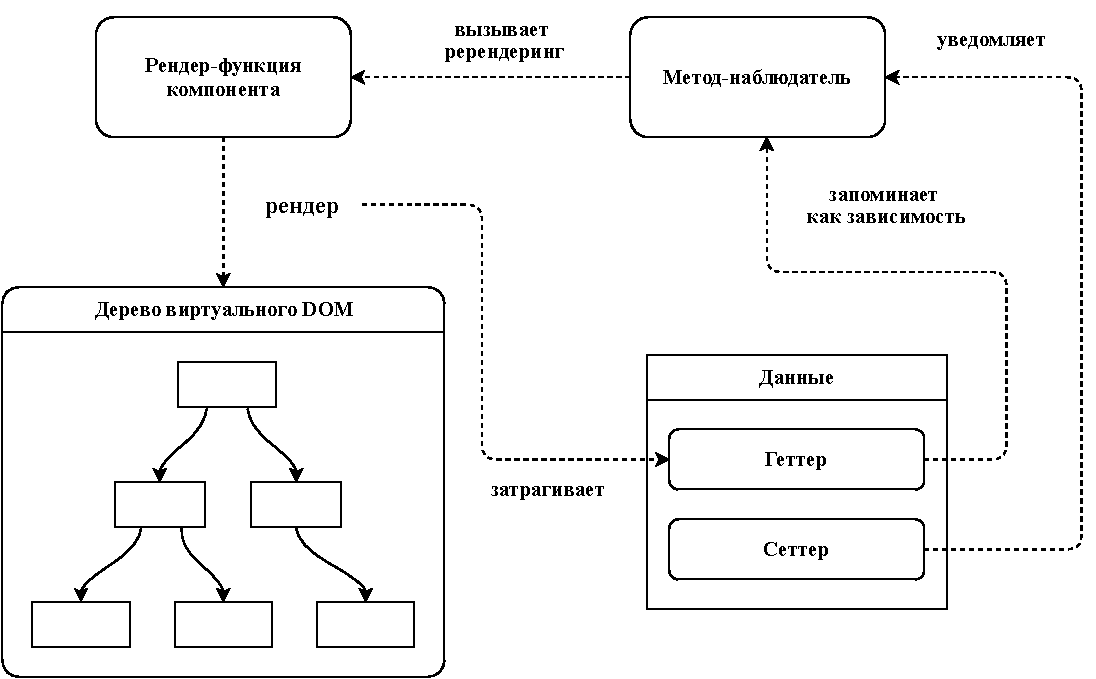
\includegraphics[width=\textwidth]{figures/reactivity}
	\caption{Визуализация работы реактивности}
	\label{fig:react}
\end{figure}

Однако у подобного способа отслеживания изменений имеется ряд особенностей и нюансов. Дело в том, что вследствие определенных ограничений JavaScript существуют такие виды изменений, которые Vue не способен обнаружить. К счастью, существуют способы обойти их и сохранить реактивность. Один из таких способов~--- метод \texttt{Vue.set}. Данный метод принимает на вход три аргумента:

\begin{itemize}
	\item объект, в который будет добавлено новое свойство;
	\item имя нового свойства либо его индекс;
	\item значение нового свойства.
\end{itemize}

Рассмотрим его на примере мутации \texttt{setUserName}, которая задает новое имя пользователя (листинг \ref{lst:vueset}). В данном случае новое свойство \texttt{name} добавляется в объект \texttt{state.user}, затем для этого свойства автоматически создается пара геттер и сеттер, которые обеспечивают его реактивность.

\lstinputlisting[
caption=Метод Vue.set,
label=lst:vueset]
{listings/vueset.txt}

\subsection{SpeechSynthesis}

Интерфейс \texttt{SpeechSynthesis} входит в состав Web Speech API и позволяет веб-приложению управлять голосовыми данными. Данная технология хоть и является экспериментальной, но уже поддерживается большинством браузеров \cite{speech}.

В разрабатываемом приложении \texttt{SpeechSynthesis} играет ключевую роль при изучении слов, ведь пользователю необходимо знать, как точно звучит слово, чтобы быть способным его произносить.

В листинге \ref{lst:speech} показаны две функции: \texttt{getVoices} для получения списка доступных голосов и функция \texttt{pronounceWord}, которая принимает на вход в качестве аргументов исходное слово для перевода и сам голос для его озвучивания.

\clearpage

\lstinputlisting[
caption=Получение списка голосов и произношение слова,
label=lst:speech]
{listings/speechSynthesis.js}

Метод \texttt{SpeechSynthesis.getVoices} возвращает список объектов \texttt{SpeechSynthesisVoice}, представляющих все доступные голоса.

Объект \texttt{SpeechSynthesisUtterance} содержит свойство текста, который будет синтезироваться при произнесении слова или высказывания, а также устанавливает определенные настройки по его звучанию (громкость, скорость, высота и голос озвучивания). Метод \texttt{SpeechSynthesis.speak} позволяет произносить полученную на вход информацию исходя из заданных настроек.

В листинге \ref{lst:words} показана инициализация \texttt{SpeechSynthesis} в компоненте. Для определенной выше в листинге \ref{lst:speech} функции \texttt{getVoices} применяется фильтр, который выбирает только английские голоса. Если хотя бы один такой голос доступен, то из этого массива голосов выбирается самый первый и кладется в переменную \texttt{voice} (сами голоса в основном различаются по полу и интонации говорящего). Для желаемого слова вызывается функция \texttt{pronounce}, которая вызывает определенный выше метод \texttt{pronounceWord} из листинга \ref{lst:speech} и озвучивает это слово заданным голосом.

\clearpage

\lstinputlisting[
caption=Инициализация SpeechSynthesis в компоненте,
label=lst:words]
{listings/userwords.vue}

\subsection{Axios}

\textbf{Axios}~--- это основанная на промисах библиотека для выполнения HTTP-запросов, которая позволяет получать и отображать данные из стороннего API.

С помощью Axios и API Яндекс.Переводчика \cite{yandex} становится возможна имплементация метода параллельного чтения, представленного в разделе 1. Синтаксис запроса для перевода текста представлен в листинге \ref{lst:yandex}. При инициализации запроса ответ возвращается в формате JSON. В таблице \ref{tab:tab2} приведено описание всех параметров, которые можно передать запросу, а в таблице \ref{tab:tab3} описаны возможные коды ответов.

\lstinputlisting[
caption=Синтаксис запроса Яндекс.Переводчика,
label=lst:yandex]
{listings/yandex.txt}

\begin{table}[h]
	\centering
	\begin{tabular}{ |c|l|c|c| }
		\hline
		Параметр & Описание \\
		\hline
		key & Бесплатный API-ключ \\
		\hline
		text & Текст, который необходимо перевести \\
		\hline
		lang & Направление перевода (например, \texttt{en-ru}) \\
		\hline
		format & Формат текста (текст без разметки или в формате HTML) \\
		\hline
		options & Опции перевода \\ 
		\hline
		callback & Имя функции обратного вызова \\ 
		\hline
	\end{tabular}
	\caption{Описание передаваемых параметров запросу}
	\label{tab:tab2}
\end{table}

\begin{table}[h]
	\centering
	\begin{tabular}{ |c|l|c|c| }
		\hline
		Значение & Описание \\
		\hline
		200 & Операция выполнена успешно \\
		\hline
		401 & Некорректный API-ключ \\
		\hline
		402 & API-ключ заблокирован \\
		\hline
		404 & Превышен суточный лимит на объем переведенного текста \\
		\hline
		413 & Превышен максимально допустимый размер текста \\ 
		\hline
		422 & Невозможно перевести текст \\ 
		\hline
		501 & Данное направление перевода не поддерживается \\ 
		\hline
	\end{tabular}
	\caption{Коды возможных ответов и их описание}
	\label{tab:tab3}
\end{table}

Имплементация метода параллельного чтения в компоненте показана в листинге \ref{lst:axios}. Он осуществляется засчет метода \texttt{window.getSelection}, который возвращает объект \texttt{Selection}, представленный в виде диапазона текста, который пользователь выделил на странице. Затем вызывается метод \texttt{getSelectedTextAndTranslate}, который осуществляет перевод выделенного текста с помощью вызова функции \texttt{getTranslation} и инициирует показ снэкбара с переводом текста.

В функции \texttt{getTranslation} осуществляется GET-запрос к API Яндекс.Переводчика с передаваемым ему фрагментом текста.

Яндекс.Переводчик использует гибридную модель машинного перевода, которая включает в себя нейросетевой и статистический подходы. Последний основан на моделях языка: исходный текст разбивается на слова и фразы, которые переводятся независимо друг от друга, после чего для каждой части текста подбирается потенциальный перевод из матрицы. Затем система выбирает лучший перевод с точки зрения сочетаемости слов в языке. Однако недостаток данного подхода в том, что не всегда удается установить взаимосвязь между фразами. И тут на помощь приходит нейросетевой подход, который позволяет учитывать контекст и добиться более связного по смыслу перевода. В отличие от статистического подхода, текст не разбивается на отдельные части, а переводится полностью. В данном подходе используется векторное представление слов (англ. \textit{word embedding}). Вектор состоит из чисел, которые характеризуют слово по семантическим и лексическим признакам. В итоге предложение представляет из себя векторное пространство, в котором нейронная сеть определяет семантику слов и взаимосвязь между ними.

Текст для перевода передается двум системам сразу, а затем на основе оценке алгоритма определяется, какой из переводов показывать пользователю. Таким образом, можно не беспокоиться о качестве перевода, т.~к. в большинстве случаев он будет относительно связным по смыслу.

\lstinputlisting[
caption=Имплементация метода параллельного чтения,
label=lst:axios]
{listings/axios.vue}

\subsection{Шина событий}

Рассмотрим такую ситуацию: пользователь решил изменить свой электронный адрес; для этого он зашел в настройки профиля, нажал на гипотетическую кнопку <<изменить>>~--- появилось модальное окно, в котором пользователь ввел новый адрес, который сервер успешно обработал. Проблема состоит в том, как же дать нашему приложению понять, в какой момент необходимо закрывать это модальное окно.

Для решения этой проблемы необходимо ввести такое понятие, как \textit{шина событий}. По сути, это экземпляр Vue, который используется для работы с событиями: он имеет возможность как имитировать события с помощью метода \texttt{\$emit}, так и подписываться на них благодаря методу \texttt{\$on} (рис.~\ref{fig:bus}).

\begin{figure}[h]
	\centering
	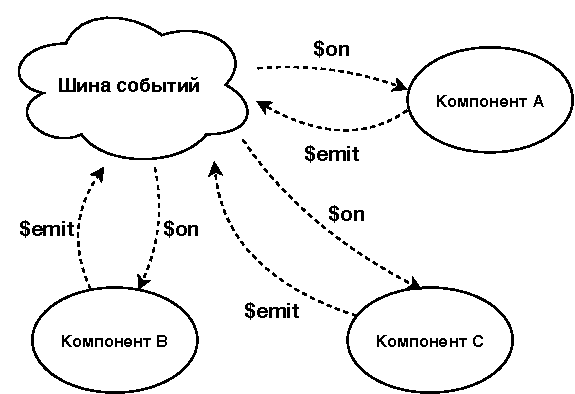
\includegraphics[width=0.85\textwidth, keepaspectratio]{figures/eventbus}
	\caption{Шина событий}
	\label{fig:bus}
\end{figure}

Создание шины событий отражено в листинге \ref{lst:bus1}. Метод \texttt{notify} можно назвать <<фасадом>> для функции \texttt{\$emit}, в то время как функция \texttt{setUpBus} на уровне прототипа Vue создает свойство \texttt{\$bus}, которое, являясь геттером, возвращает объект \texttt{EventBus}.

\clearpage

\lstinputlisting[
caption=Инициализация шины событий,
label=lst:bus1]
{listings/eventbus.js}

Затем в компоненте, который предназначен для изменения пользовательских данных и содержит в себе то самое незакрытое модальное окно, создадим хук \texttt{created}, в котором подпишемся на событие \texttt{useremail:changed}, а функциональность самого события будет заключаться в переключении значения переменной \texttt{userEmailDialog}; также для устранения утечки памяти стоит отписываться от события перед уничтожением экземпляра Vue, используя хуки \texttt{beforeDestroy} и метод \texttt{\$off} (листинг \ref{lst:bus2}).

Все, что осталось сделать,~--- имитировать это событие. События можно имитировать как из мутаций, так и напрямую из действий. В листинге \ref{lst:bus3} это делается через мутацию \texttt{setUserEmail}, отвечающую за изменение электронной почты пользователя. Теперь модальное окно закроется сразу как только имитируется данное событие.

Стоит отметить, что шина событий используется во многих частях разрабатываемого приложения: например, когда необходимо уведомить компонент об изменении состояния и отрисовать новое представление в ответ на определенный <<триггер>>.

\clearpage

\lstinputlisting[
caption=Подписка на событие в компоненте,
label=lst:bus2]
{listings/eventbus2.vue}

\lstinputlisting[
caption=Имитация события,
label=lst:bus3]
{listings/eventbus3.js}

\section{Серверная часть приложения}

\subsection{Структура базы данных}

Для хранения данных Cloud Firestore использует документы и коллекции. Если провести аналогию с системой управления баз данных реляционного типа (например, MySQL, PostgreSQL, Access, Oracle и т.~д.), то коллекция~--- это таблица, а документ является записью в этой таблице. Одна коллекция состоит из множества документов, которые содержат в себе набор полей или даже вложенные коллекции.

Структура всех коллекций базы данных для разрабатываемого приложения доступна в приложении А. С учетом того, что Cloud Firestore предоставляет возможность создания вложенных коллекций, следует уточнить, почему коллекция \textit{bookParts} (рис.~\ref{fig:bookPartsDiagram}) не была объявлена вложенной коллекцией для коллекции \textit{books} (рис.~\ref{fig:booksDiagram}). Дело в том, что при вызове одной коллекции также вызываются все ее вложенные коллекции, что неблагоприятно сказывается на оптимизации приложения. Таким образом, мы подсознательно идем на дубликацию некоторых данных, чтобы вытащить необходимые нам данные одним запросом. Учитывая то, что тарифный план Firebase имеет лимит на запросы для использования бесплатного режима (максимум 50 тыс. запросов на чтение в сутки), это является наиболее оптимальным и правильным решением.

\subsection{Правила базы данных}

Правила в Cloud Firestore обеспечивают контроль доступа к определенным коллекциям и документам и позволяют разработчику сосредоточиться на создании удобного пользовательского интерфейса без необходимости управления инфраструктурой или написания дополнительного кода на стороне сервера. 

Любое правило состоит из оператора \texttt{match}, которое идентифицирует документы в базе данных, а также из выражения \texttt{allow}, которое контролирует доступ к этим документам. Синтаксис для правила представлен в листинге \ref{lst:rule}.

\lstinputlisting[
caption=Синтаксис правила в Cloud Firestore,
label=lst:rule]
{listings/rule.txt}

Правила для разрабатываемого приложения представлены в листинге \ref{lst:rules}. Дадим некоторые пояснения:

\begin{itemize}
	\item функция \texttt{isSignedIn} определяет, авторизован ли пользователь;
	\item функция \texttt{isAdmin} определяет, является ли пользователь администратором веб-приложения;
	\item функция \texttt{isContentOwner} определяет, является ли пользователь автором заданного контента;
	\item любой документ из коллекции \textit{books} читать могут все пользователи, а писать в любой документ из данной коллекции имеет право только администратор;
	\item любой документ из коллекции \textit{articles} читать могут все пользователи, а писать в любой конкретно заданный документ из данной коллекции имеет право либо администратор, либо создатель документа;
	\item любой документ из коллекции \textit{forum} читать могут все пользователи, а писать в любой конкретно заданный документ из данной коллекции имеет право либо администратор, либо создатель документа;
	\item любой документ из коллекции \textit{users} читать могут все пользователи, а писать в любой конкретно заданный документ из данной коллекции имеет право либо администратор, либо конкретный пользователь с заданным уникальным идентификатором;
	\item любой документ из коллекции \textit{bookParts} читать могут только те пользователи, которые добавили их в свою пользовательскую коллекцию, а писать в любой документ из данной коллекции имеет право только администратор;
	\item любой документ из коллекции \textit{userdata} доступен для чтения и редактирования только для тех пользователей, чей уникальный идентификатор совпадает с именем документа.
\end{itemize}

Путь \verb|{document=**}|, который объявлен в некоторых правилах в листинге \ref{lst:rules}, соответствует любому документу в заданной коллекции. Оператор \texttt{read} определяет доступ к документу, а оператор \texttt{write} позволяет вносить изменения в заданный документ.

\clearpage

\lstinputlisting[
caption=Правила для разрабатываемого приложения,
label=lst:rules]
{listings/rules.txt}

\clearpage

\section{Вывод}

Результатом работы в рамках данного раздела является решение следующих задач:

\begin{itemize}
	\item было подготовлено окружение для разработки, которое позволило использовать актуальные на момент написания данного проекта технологии при создании веб-приложения;
	\item было создано адаптивное и соответствующее всем заявленным требованиям веб-приложение;
	\item были описаны основные модули приложения, а также детально изложена структура клиентской и серверной частей проекта.
\end{itemize}

%%% Local Variables:
%%% mode: latex
%%% TeX-master: "rpz"
%%% End:


\backmatter %% Здесь заканчивается нумерованная часть документа и начинаются ссылки и
            %% заключение

\Conclusion % заключение к отчёту

Конечным результатом данной работы является реактивное веб-приложение для изучения иностранного языка. В рамках проведенной работы были достигнуты следующие результаты:

\begin{itemize}
	\item проведен обзор современных сервисов-аналогов, предоставляющих возможность изучения иностранного языка, функционал которых был рассмотрен и учтен при разработке собственного решения;
	\item сформулированы основные требования к веб-приложению на основе проведенного анализа предметной области с учетом используемых инструментов разработки;
	\item спроектирована архитектура веб-приложения, которая удовлетворяет всем заявленным требованиям;
	\item для приложения были реализованы все необходимые модули и компоненты, которые гарантируют работоспособность приложения;
	\item рассмотрены <<внутренности>> фреймворка Vue.js~--- в частности, были затронуты вопросы работы реактивности, подхода к управлению состоянием и имитаций событий;
	\item имплементирована логика методов для изучения иностранного языка, которые вошли в основу разработанного решения;
	\item разработана структура облачной базы данных, а также прописаны правила контроля доступа к ней.
\end{itemize}

Пользовательский интерфейс разработанного веб-приложения доступен в приложении Б.

Наиболее очевидным вариантом для улучшения разработанного решения является возможность поддержки нескольких иностранных языков: на данный момент в приложении доступен только английский.

Разработанное веб-приложение пригодно для внедрения в образовательные классы в педагогических целях.

%%% Local Variables: 
%%% mode: latex
%%% TeX-master: "rpz"
%%% End: 


% % Список литературы при помощи BibTeX
% Юзать так:
%
% pdflatex rpz
% bibtex rpz
% pdflatex rpz

\bibliographystyle{ugost2008}
\bibliography{rpz}

%%% Local Variables: 
%%% mode: latex
%%% TeX-master: "rpz"
%%% End: 


\appendix   % Тут идут приложения

\chapter{Структура Cloud Firestore}
\label{cha:appendix1}

\begin{figure}[h]
	\centering
	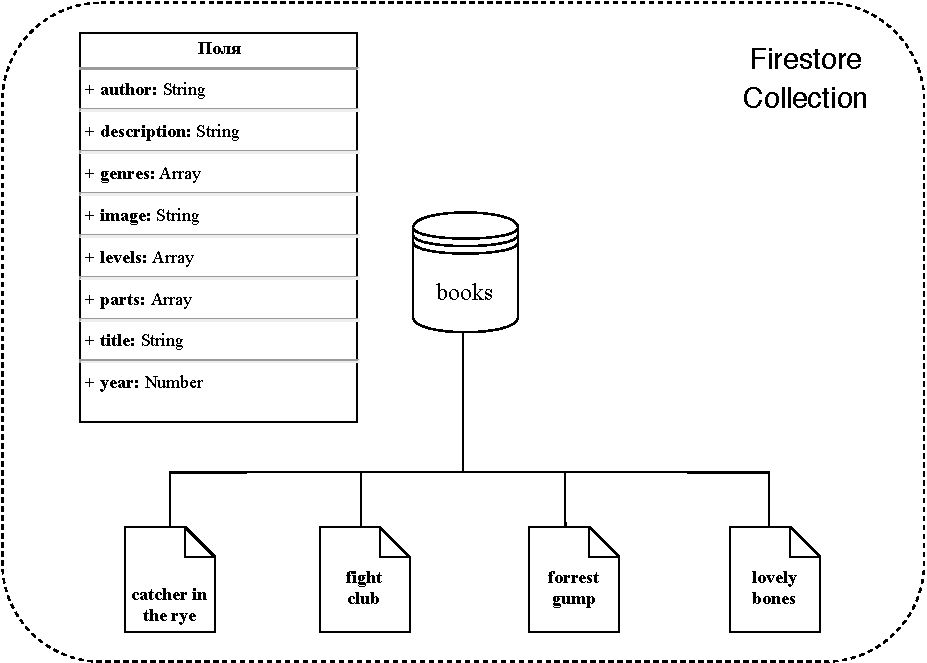
\includegraphics[width=\textwidth, keepaspectratio]{figures/books}
	\caption{Структура коллекции books}
	\label{fig:booksDiagram}
\end{figure}

\begin{figure}[h]
	\centering
	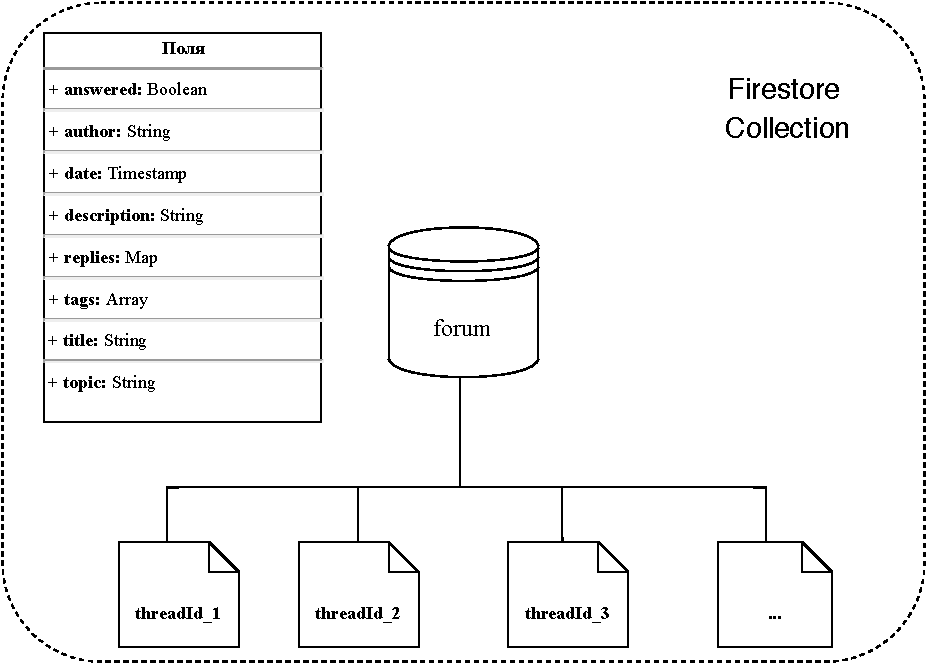
\includegraphics[width=\textwidth, keepaspectratio]{figures/forum}
	\caption{Структура коллекции forum}
	\label{fig:forumDiagram}
\end{figure}

\begin{figure}[h]
	\centering
	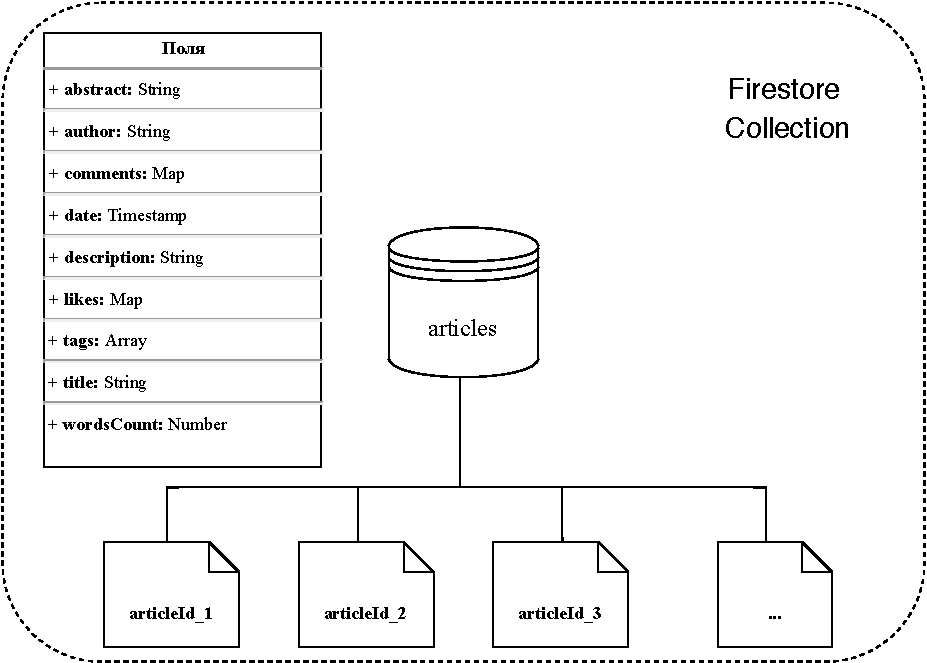
\includegraphics[width=\textwidth, keepaspectratio]{figures/articles}
	\caption{Структура коллекции articles}
	\label{fig:articlesDiagram}
\end{figure}

\begin{figure}[h]
	\centering
	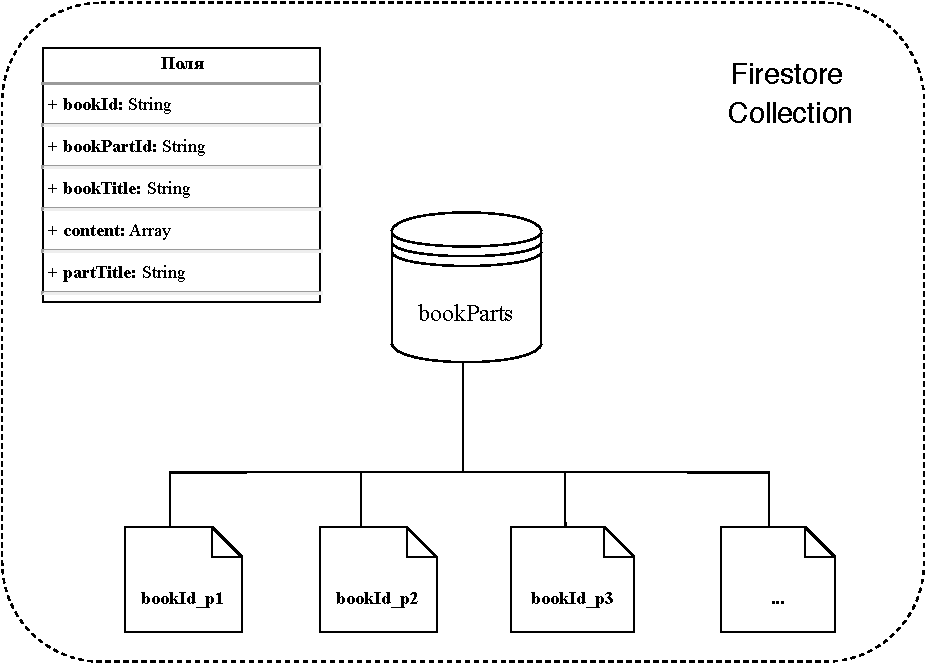
\includegraphics[width=\textwidth, keepaspectratio]{figures/bookpart}
	\caption{Структура коллекции bookParts}
	\label{fig:bookPartsDiagram}
\end{figure}

\begin{figure}[h]
	\centering
	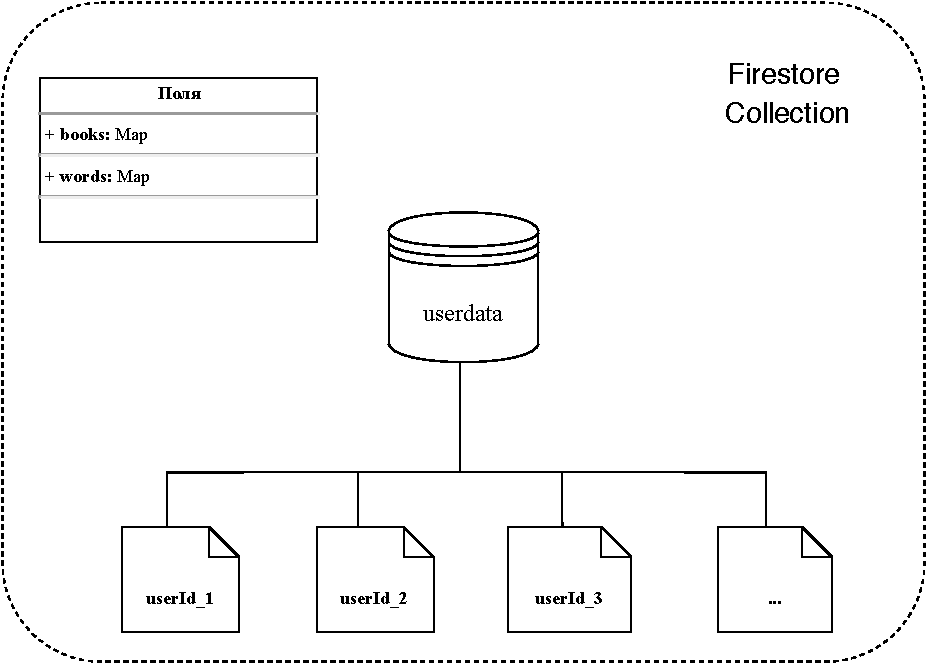
\includegraphics[width=\textwidth, keepaspectratio]{figures/userdata}
	\caption{Структура коллекции userdata}
	\label{fig:userdataDiagram}
\end{figure}

\begin{figure}[h]
	\centering
	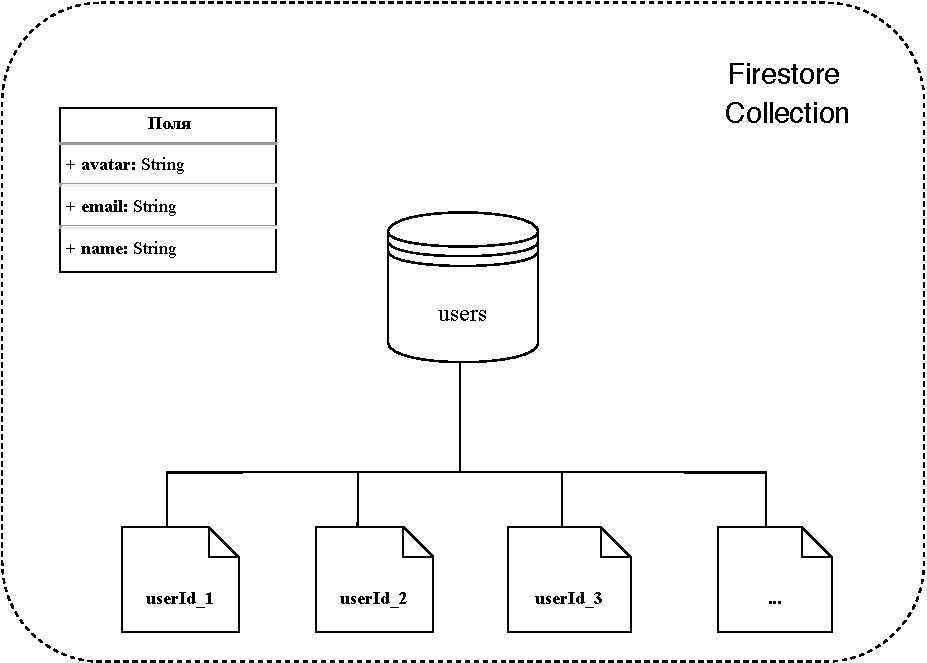
\includegraphics[width=\textwidth, keepaspectratio]{figures/users}
	\caption{Структура коллекции users}
	\label{fig:usersDiagram}
\end{figure}

%%% Local Variables: 
%%% mode: latex
%%% TeX-master: "rpz"
%%% End: 

\chapter{Интерфейс приложения}
\label{cha:appendix2}

\begin{figure}[h]
	\centering
	
\includegraphics[width=\textwidth]{figures/start}
	\caption{Стартовая страница веб-приложения}
	\label{fig:start}
\end{figure}

\begin{figure}[h]
	\centering
	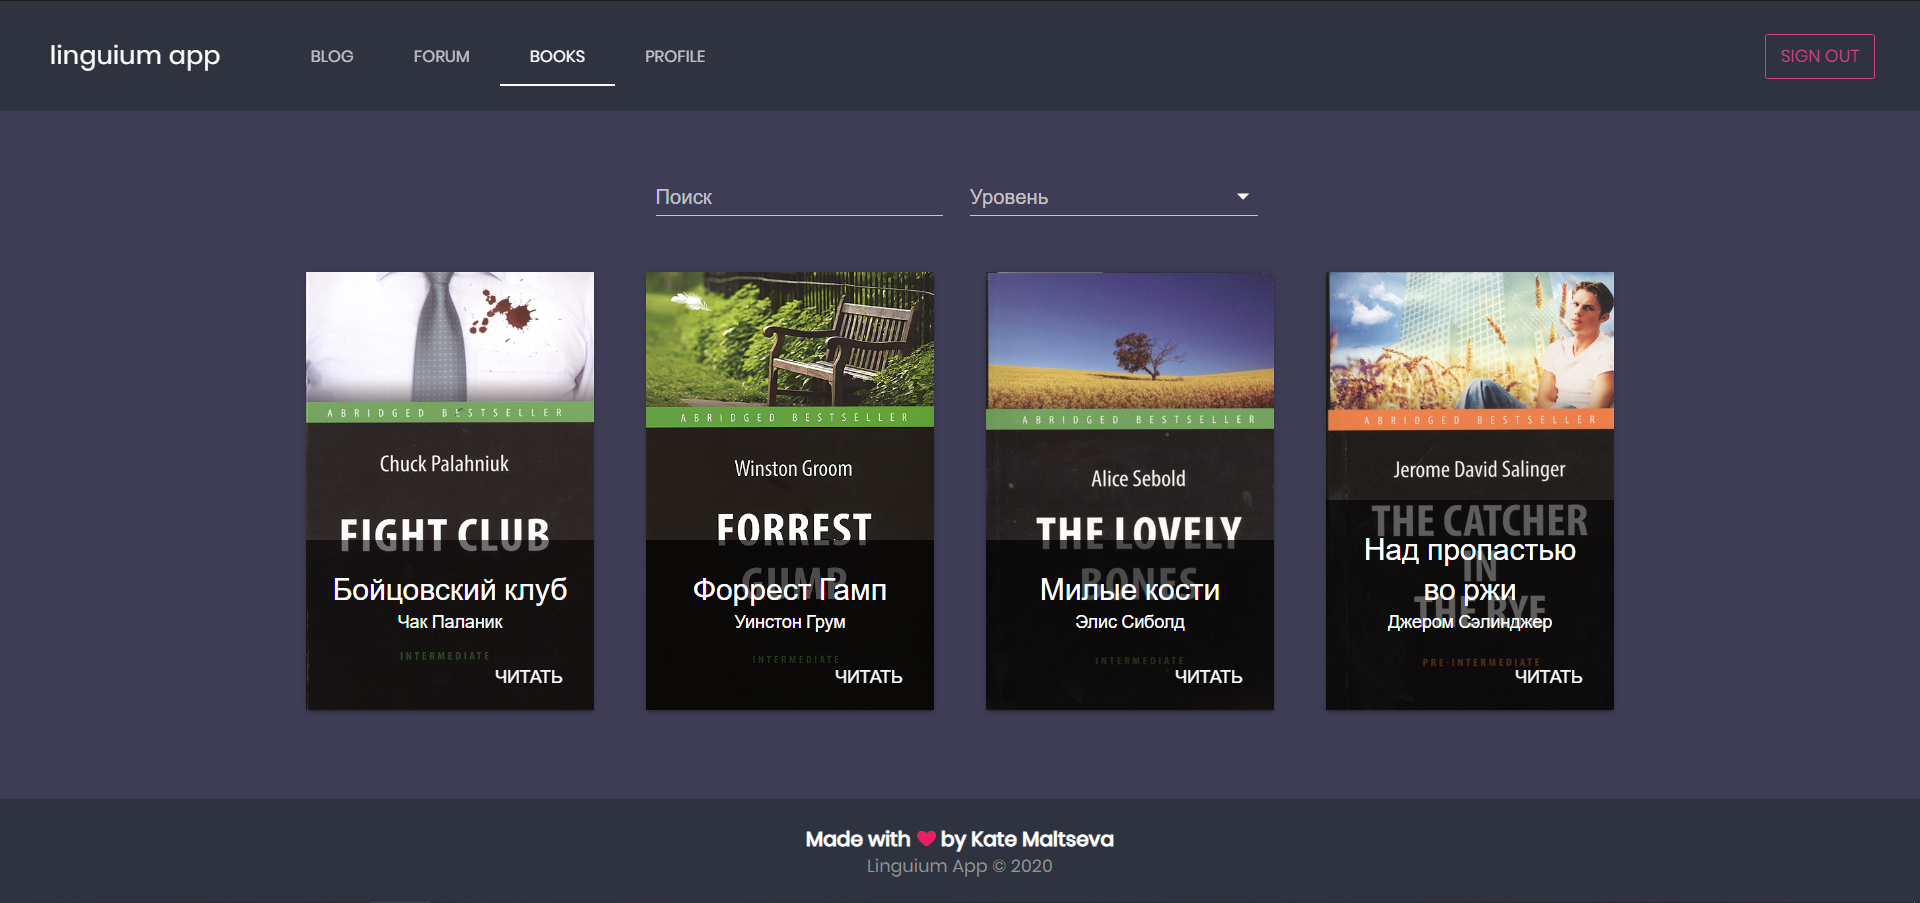
\includegraphics[width=\textwidth]{figures/booklist}
	\caption{Список доступных в приложении книг}
	\label{fig:booklist}
\end{figure}

\begin{figure}[h]
	\centering
	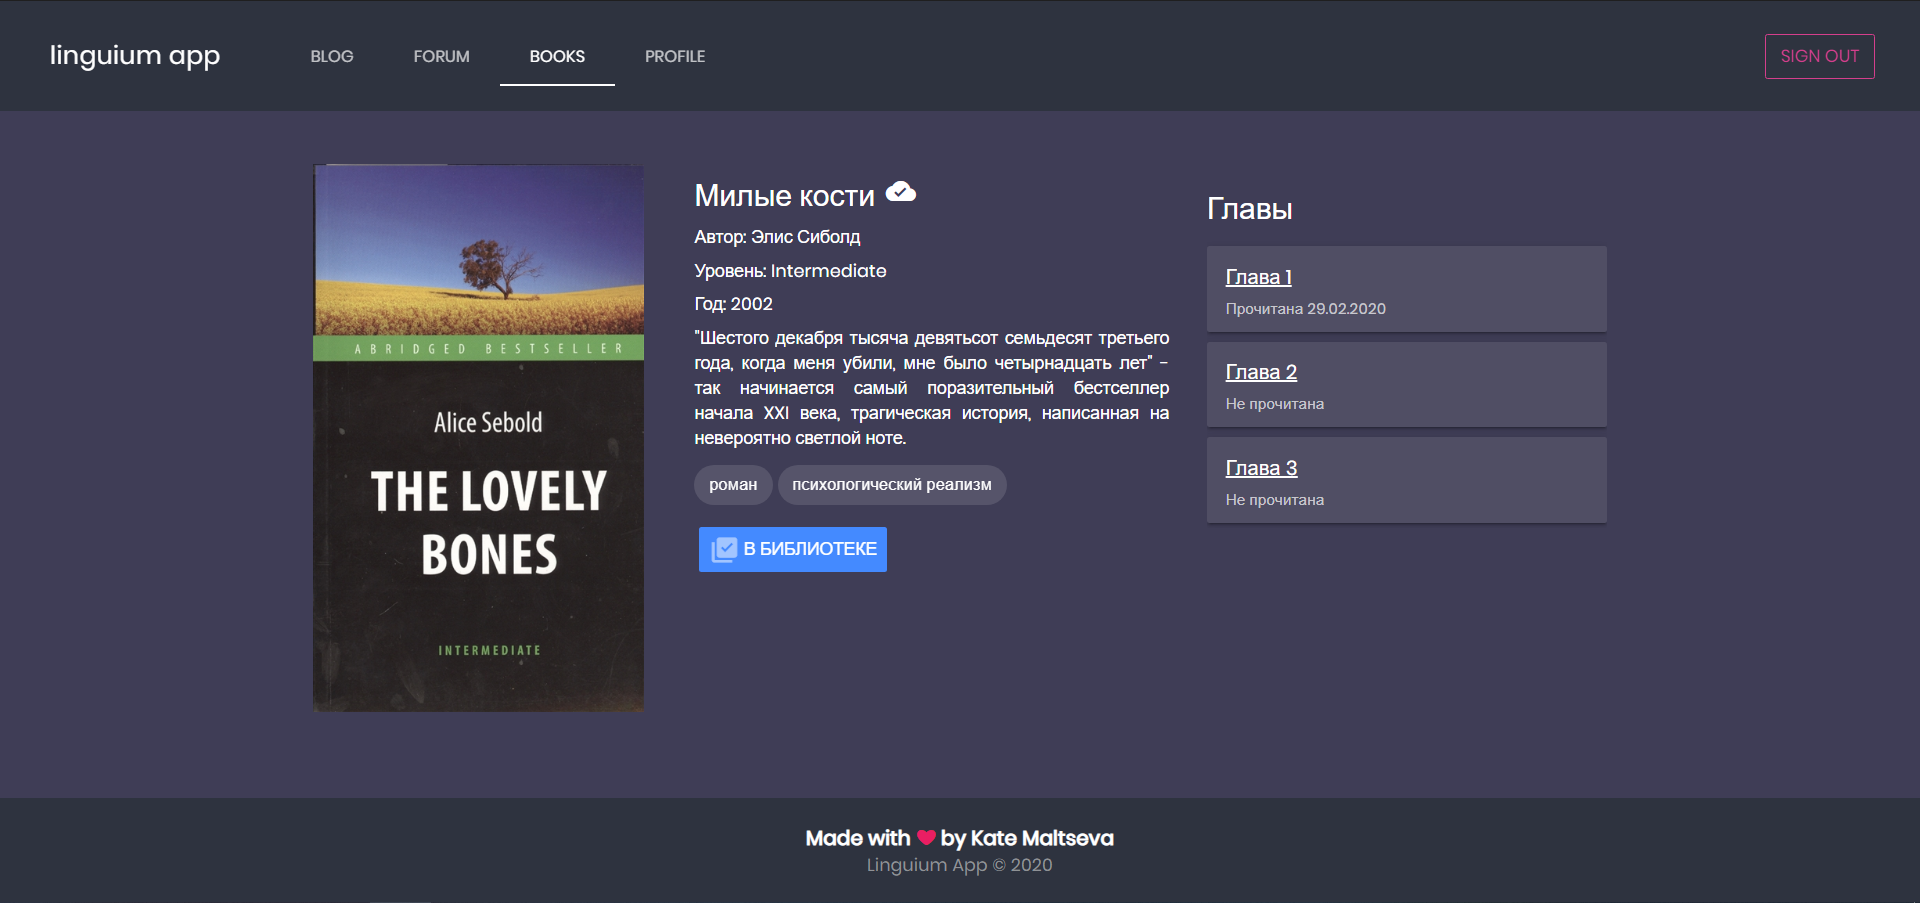
\includegraphics[width=\textwidth]{figures/bookitem}
	\caption{Информация о конкретно взятой книге и ее частях}
	\label{fig:bookitem}
\end{figure}

\begin{figure}[h]
	\centering
	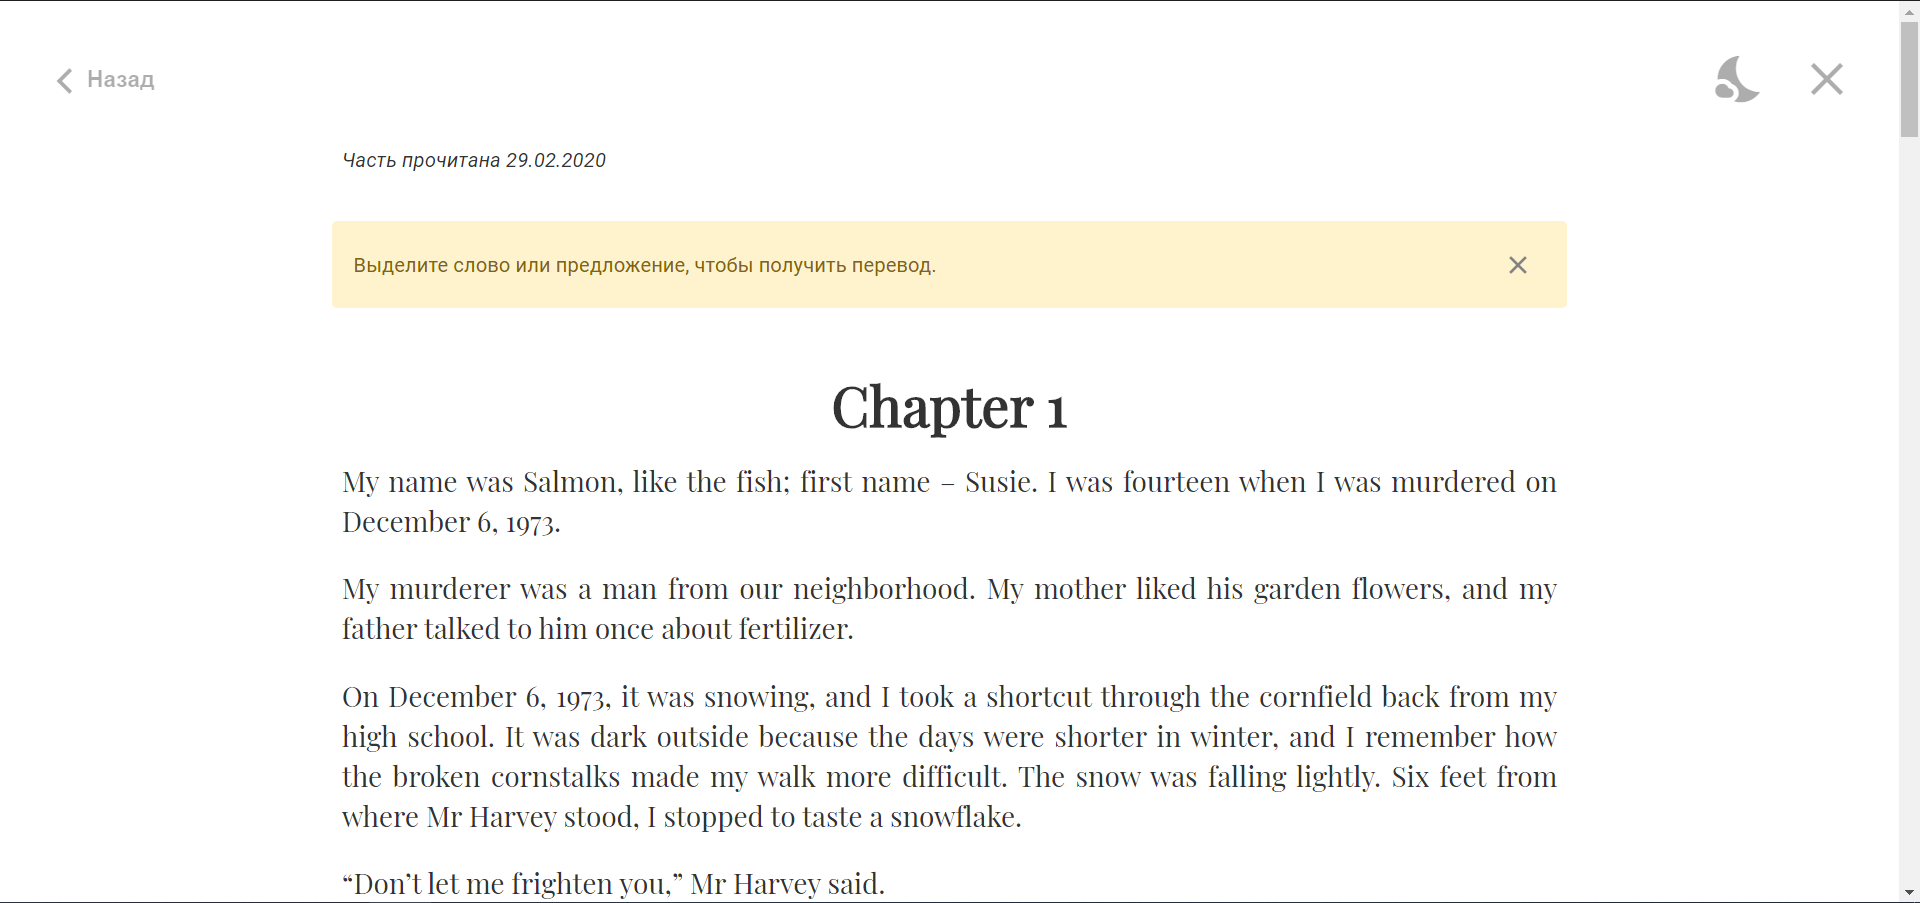
\includegraphics[width=\textwidth]{figures/reading}
	\caption{Режим чтения части книги с возможностью перевода текста и переключения темы}
	\label{fig:reading}
\end{figure}

\begin{figure}[h]
	\centering
	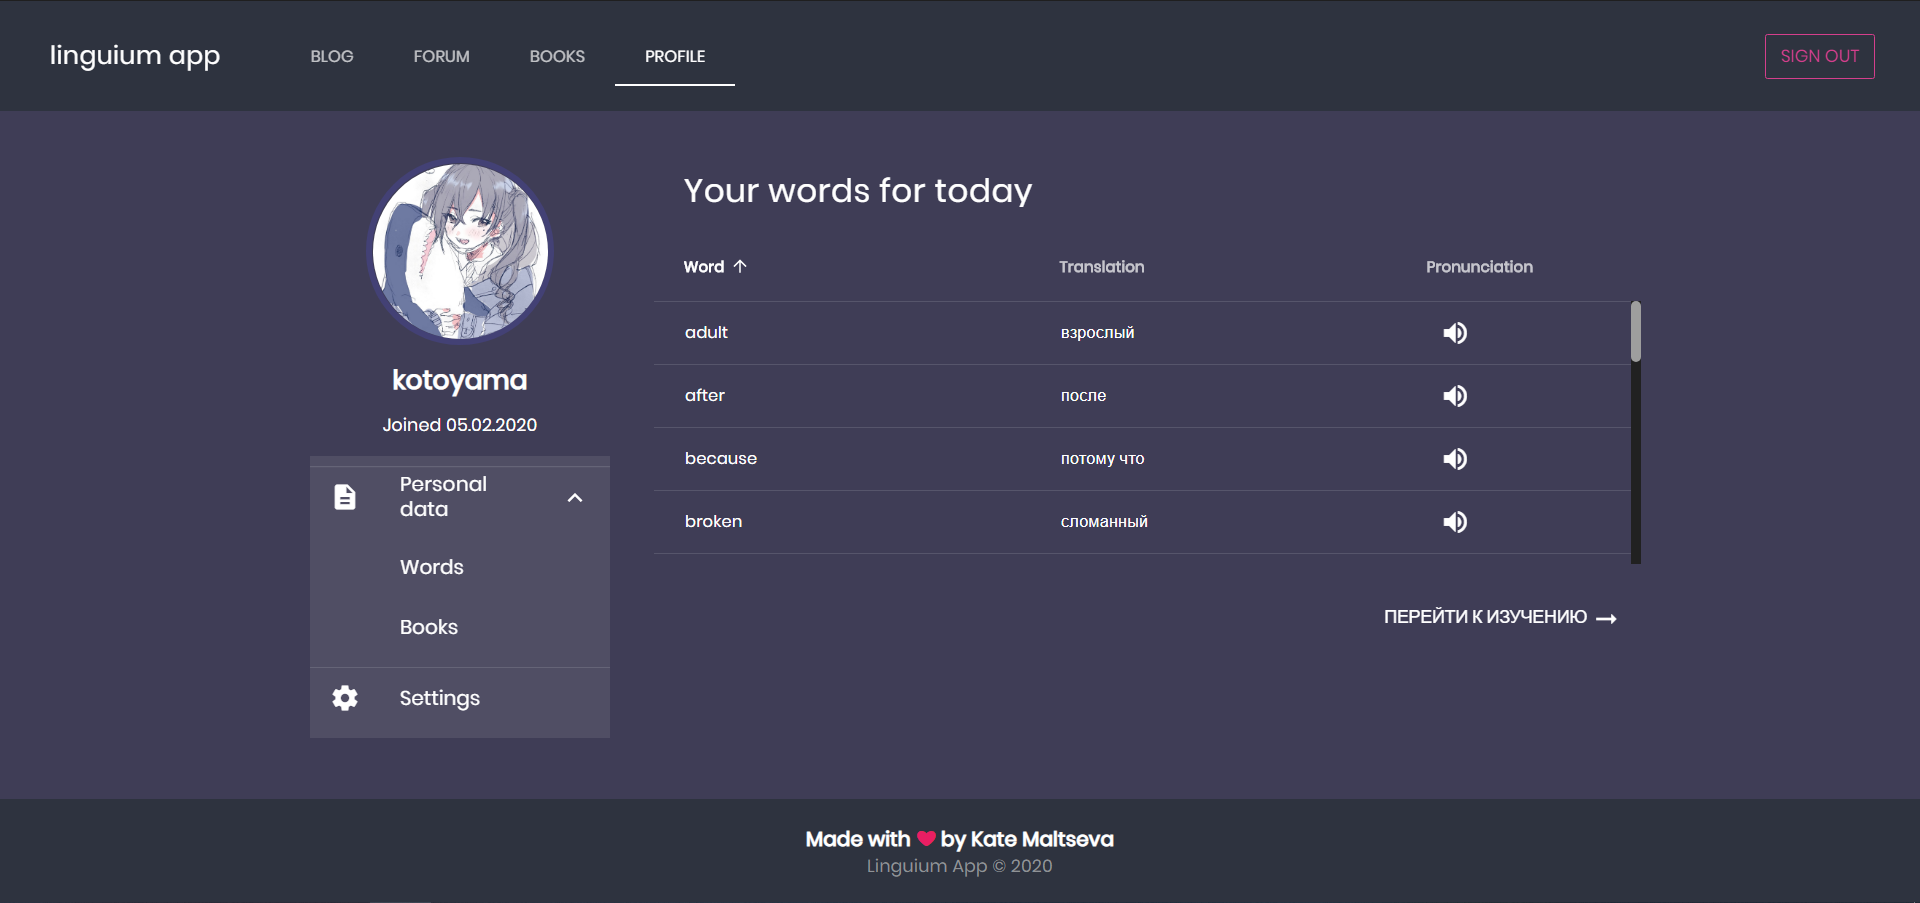
\includegraphics[width=\textwidth]{figures/profile}
	\caption{Личный кабинет пользователя со всеми его данными и возможностью настройки пользовательских данных}
	\label{fig:profile}
\end{figure}

\begin{figure}[h]
	\centering
	
\includegraphics[width=\textwidth]{figures/articlelist}
	\caption{Список статей с возможностью их фильтрации}
	\label{fig:articlelist}
\end{figure}

\begin{figure}[h]
	\centering
	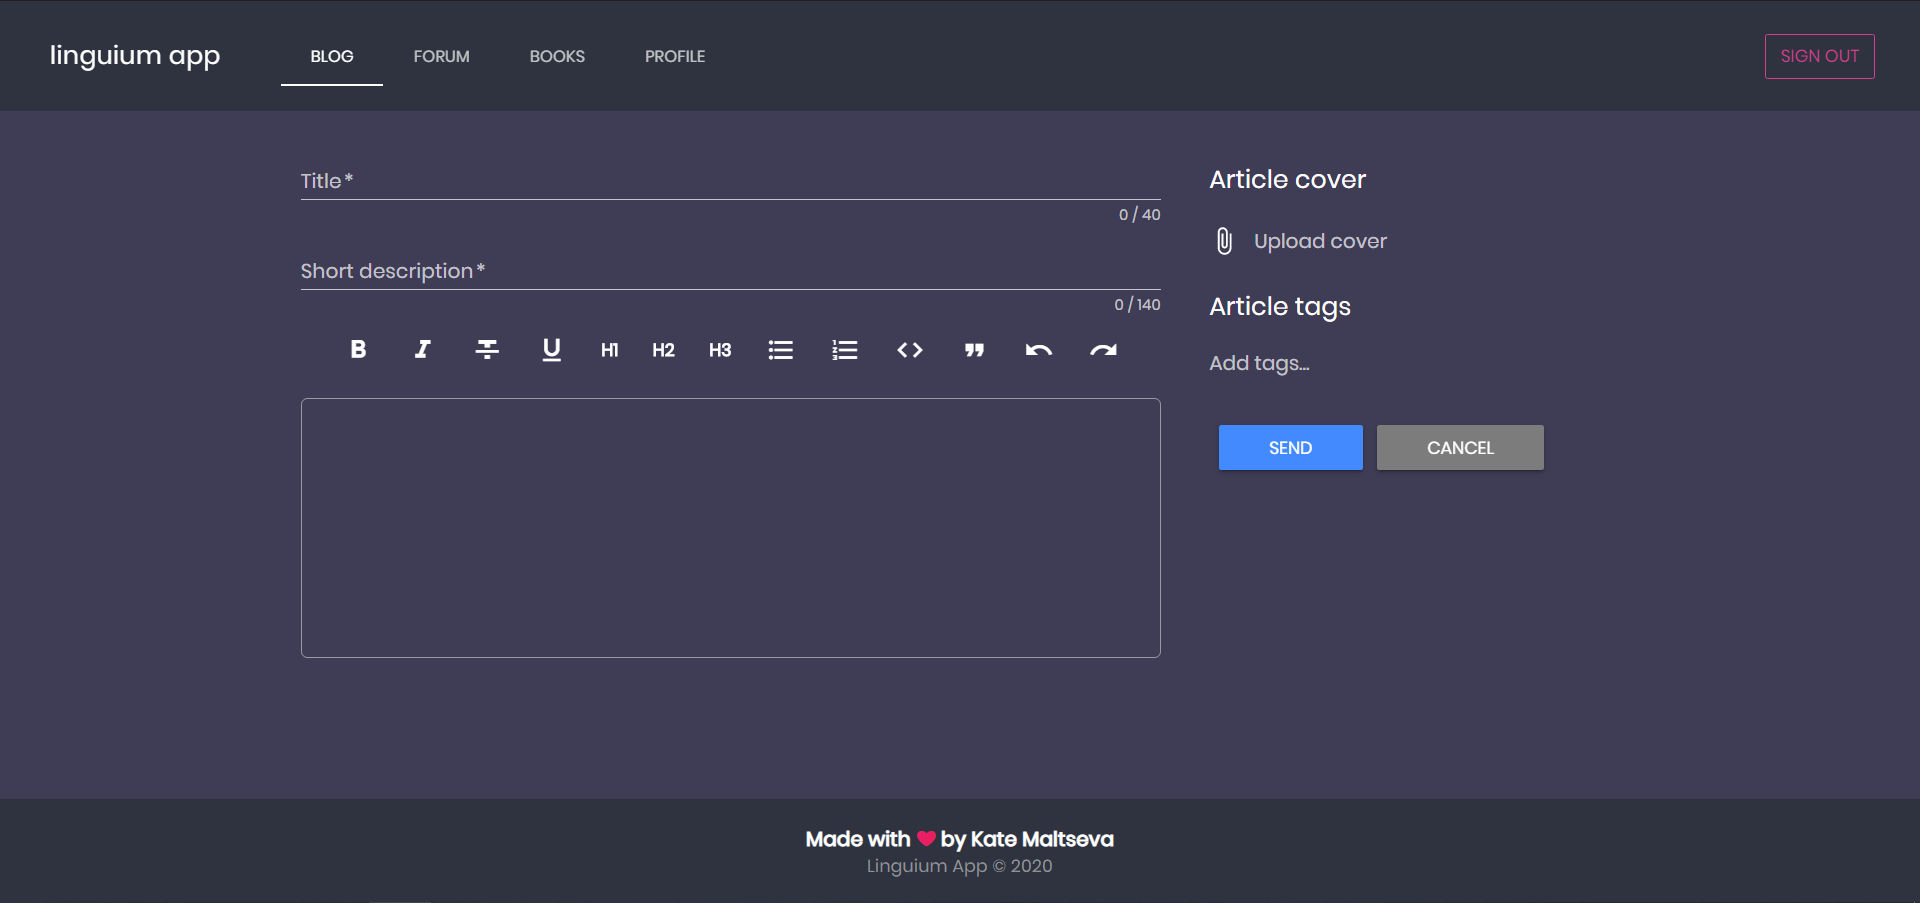
\includegraphics[width=\textwidth]{figures/createlist}
	\caption{Страница создания статьи с возможностью продвинутой верстки контента (страница для редакторования выглядит аналогичным образом)}
	\label{fig:createlist}
\end{figure}

\begin{figure}[h]
	\centering
	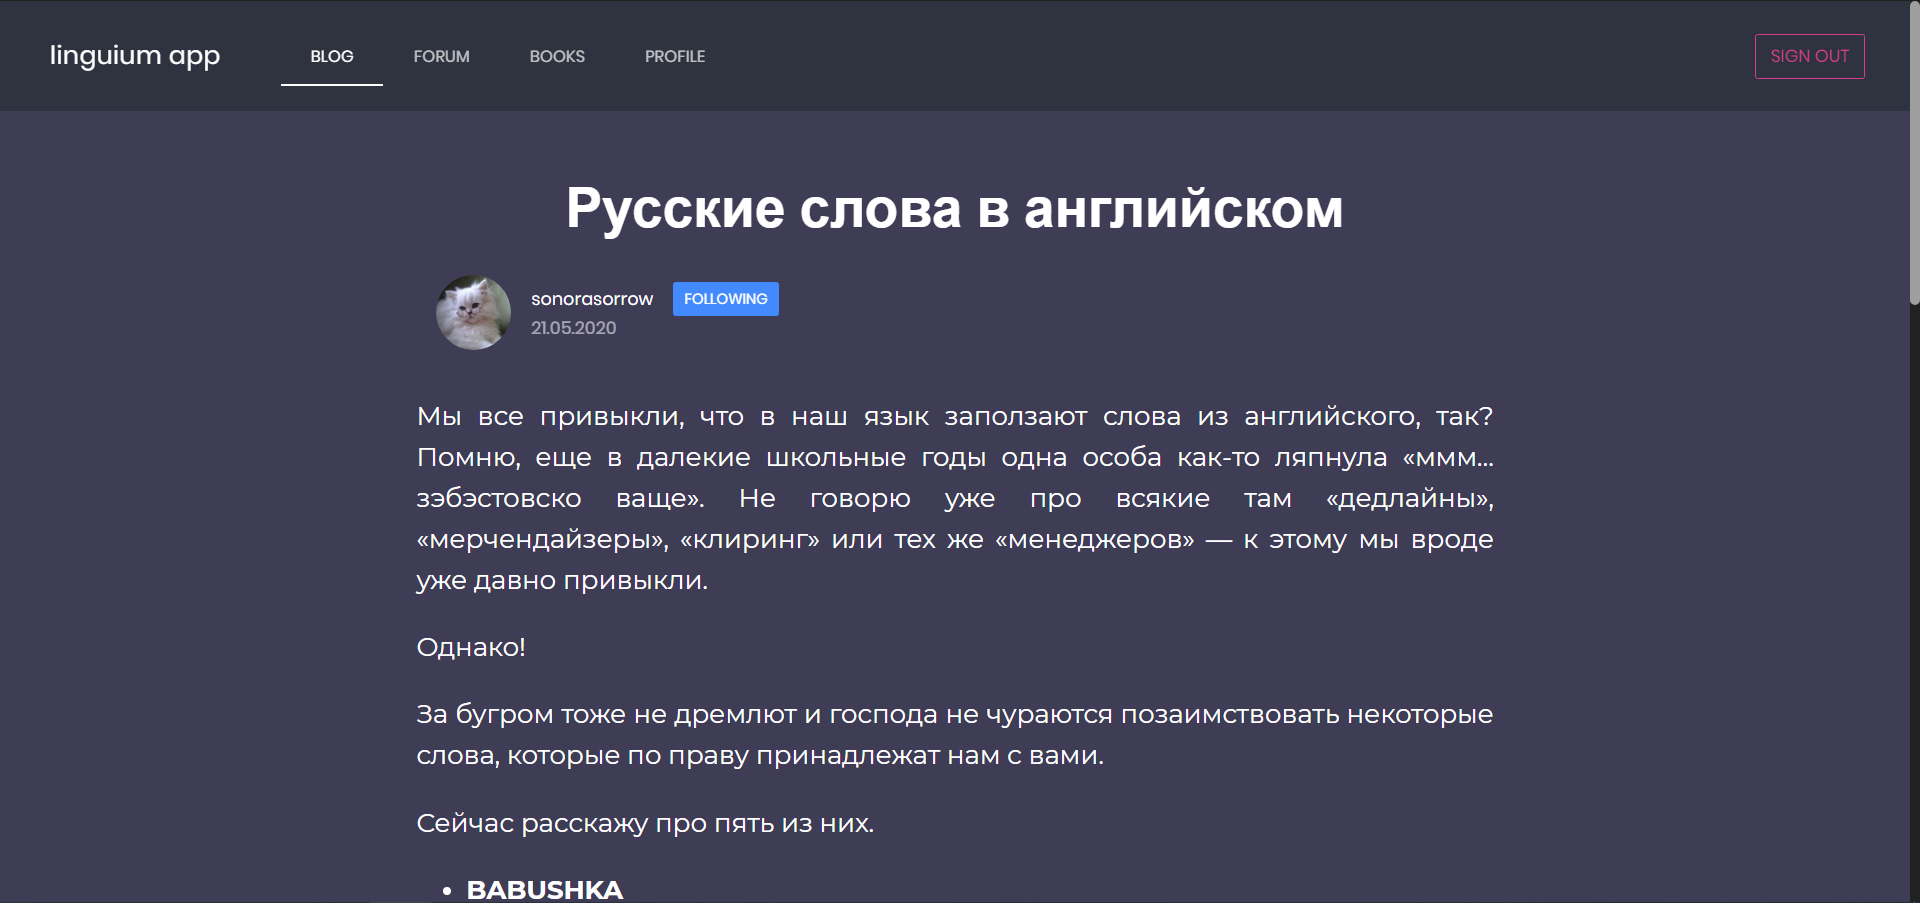
\includegraphics[width=\textwidth]{figures/articleitem}
	\caption{Содержимое конкретно взятой статьи}
	\label{fig:articleitem}
\end{figure}

\begin{figure}[h]
	\centering
	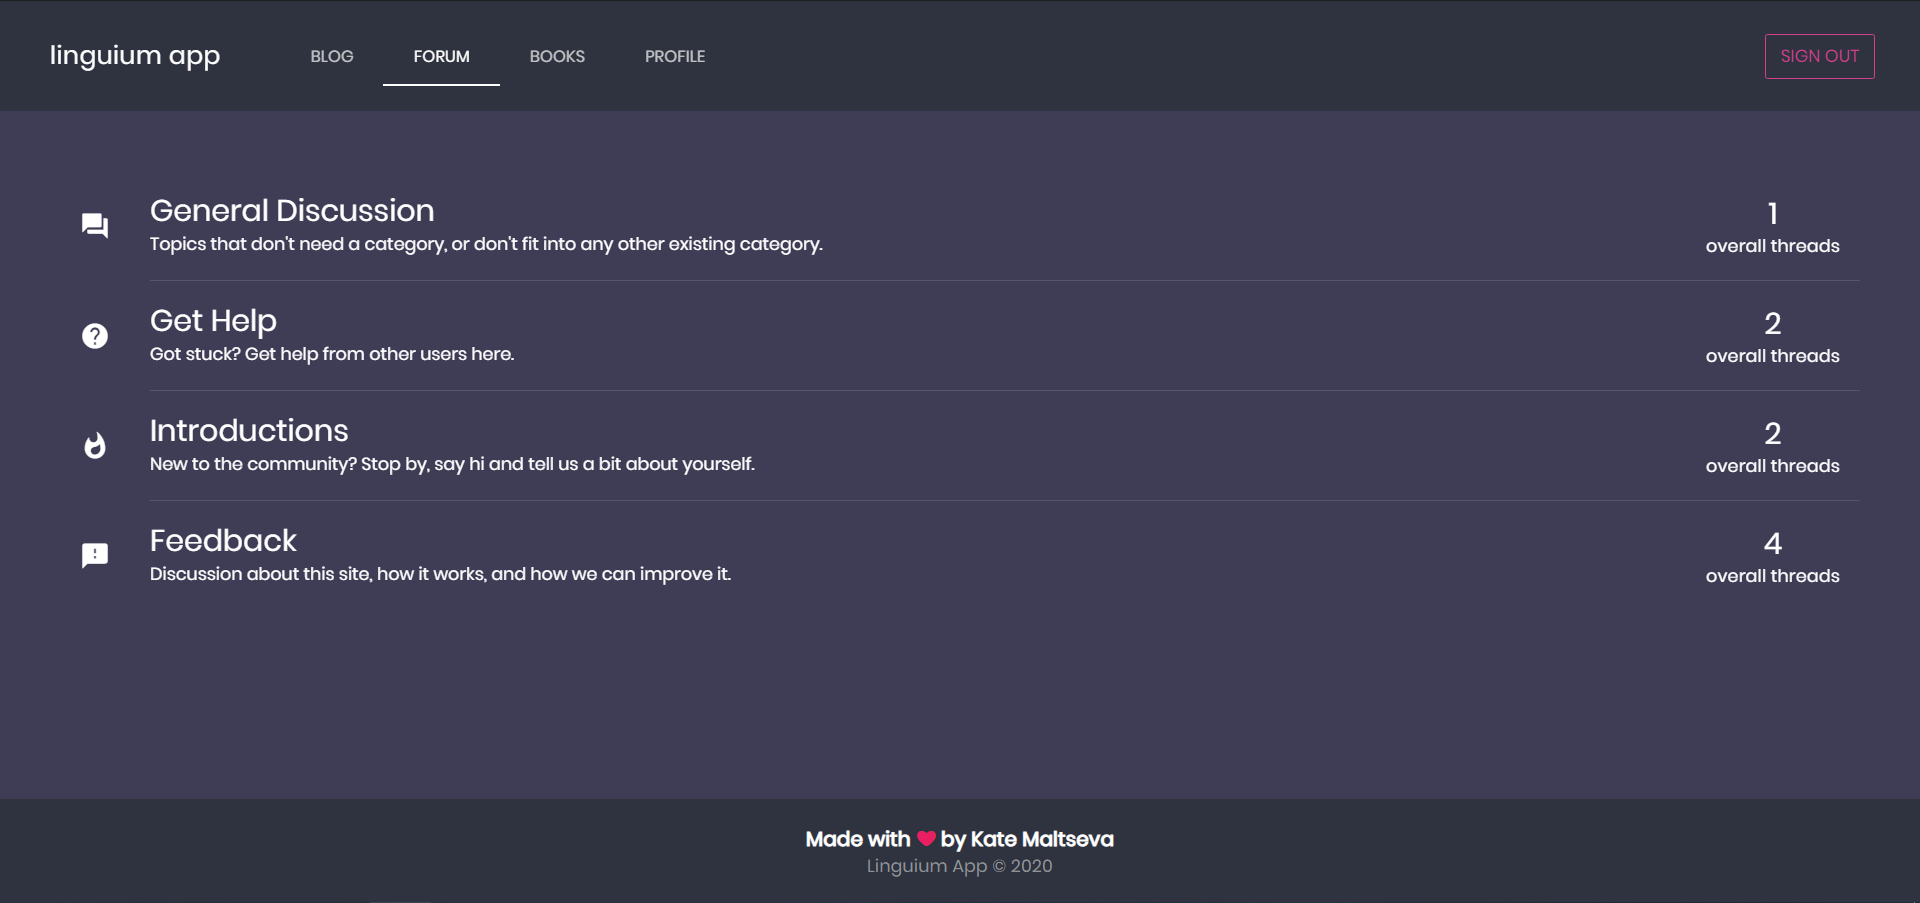
\includegraphics[width=\textwidth]{figures/forumlist}
	\caption{Форум: список всех доступных разделов и описание к ним}
	\label{fig:forumlist}
\end{figure}

\begin{figure}[h]
	\centering
	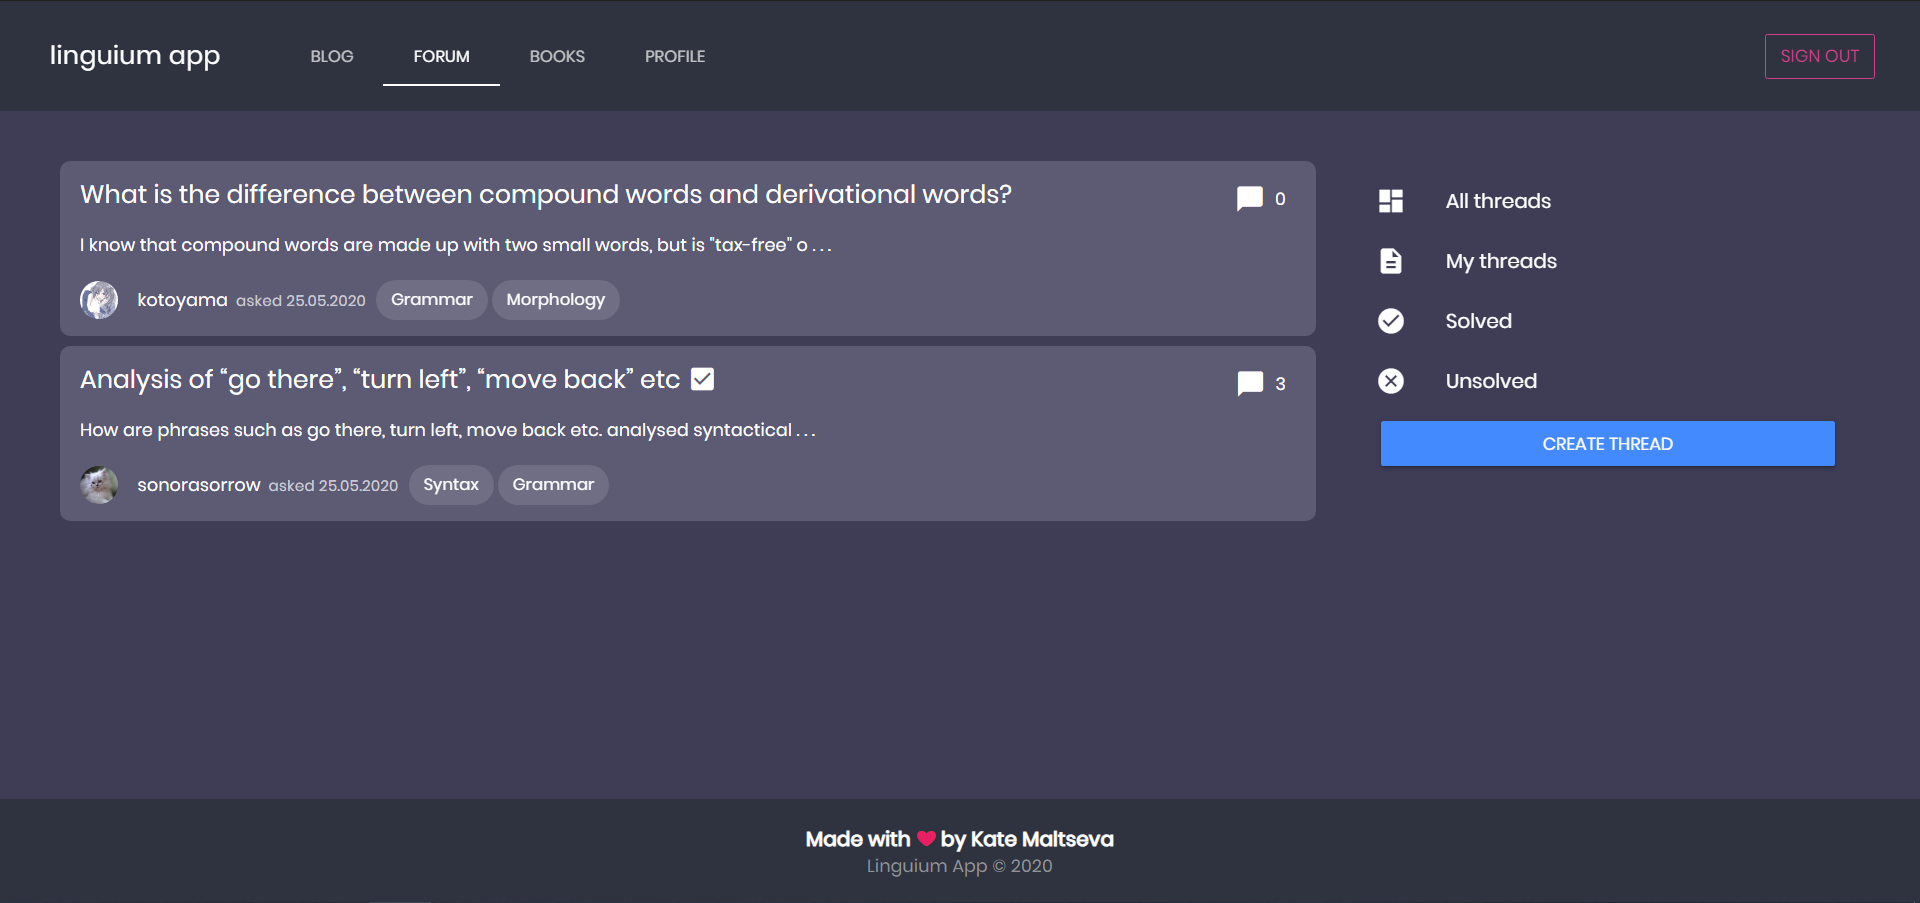
\includegraphics[width=\textwidth]{figures/topic}
	\caption{Список тредов к конкретно заданному разделу}
	\label{fig:topic}
\end{figure}

\begin{figure}[h]
	\centering
	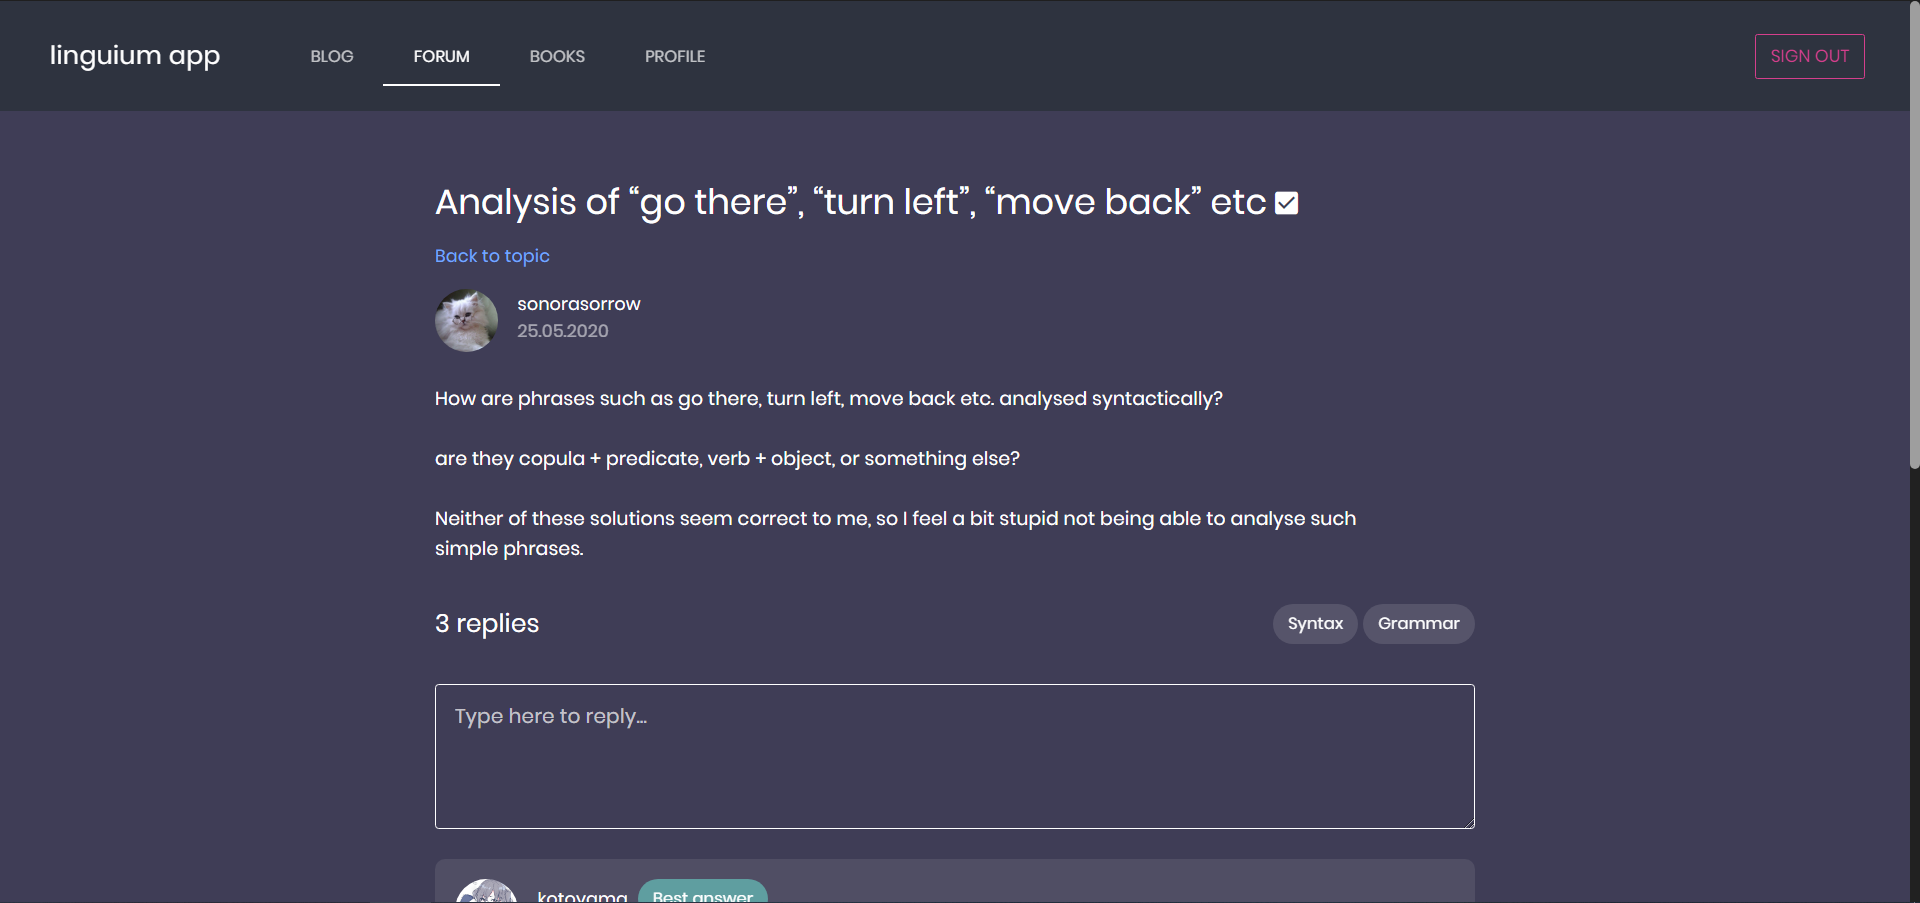
\includegraphics[width=\textwidth]{figures/thread}
	\caption{Содержимое конкретно заданного треда}
	\label{fig:thread}
\end{figure}

\begin{figure}[h]
	\centering
	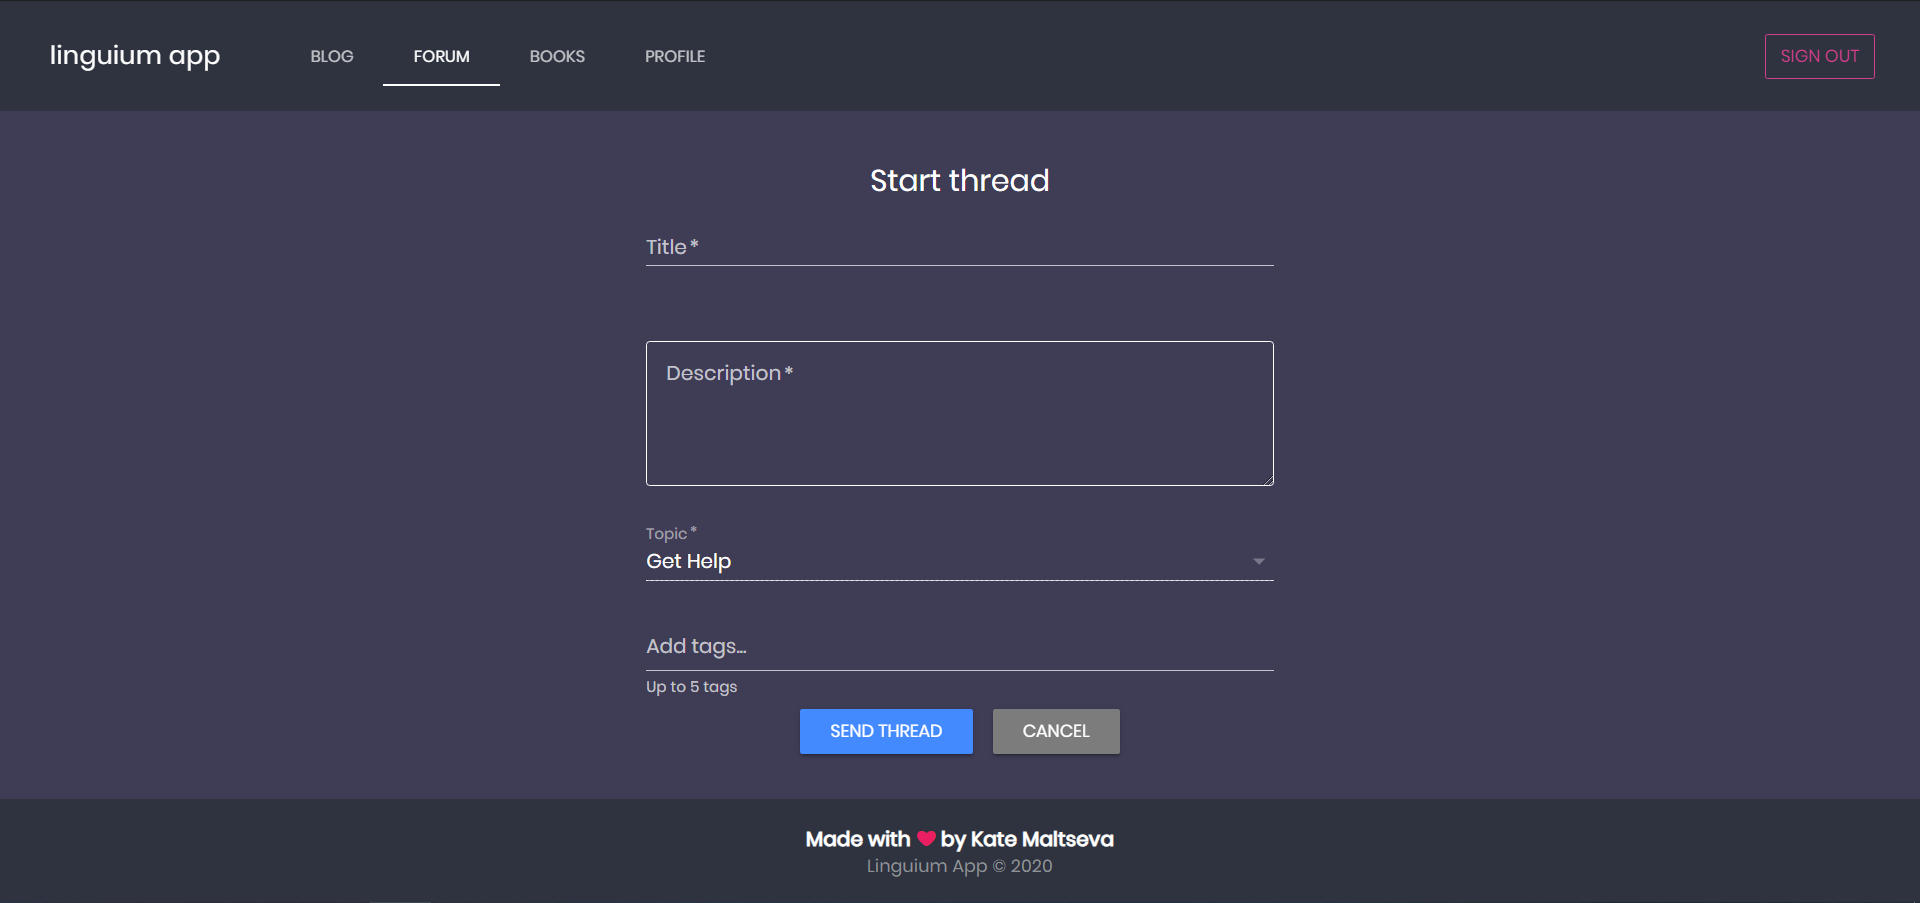
\includegraphics[width=\textwidth]{figures/createthread}
	\caption{Страница создания треда (страница для редакторования выглядит аналогичным образом)}
	\label{fig:createthread}
\end{figure}

\begin{figure}[h]
	\centering
	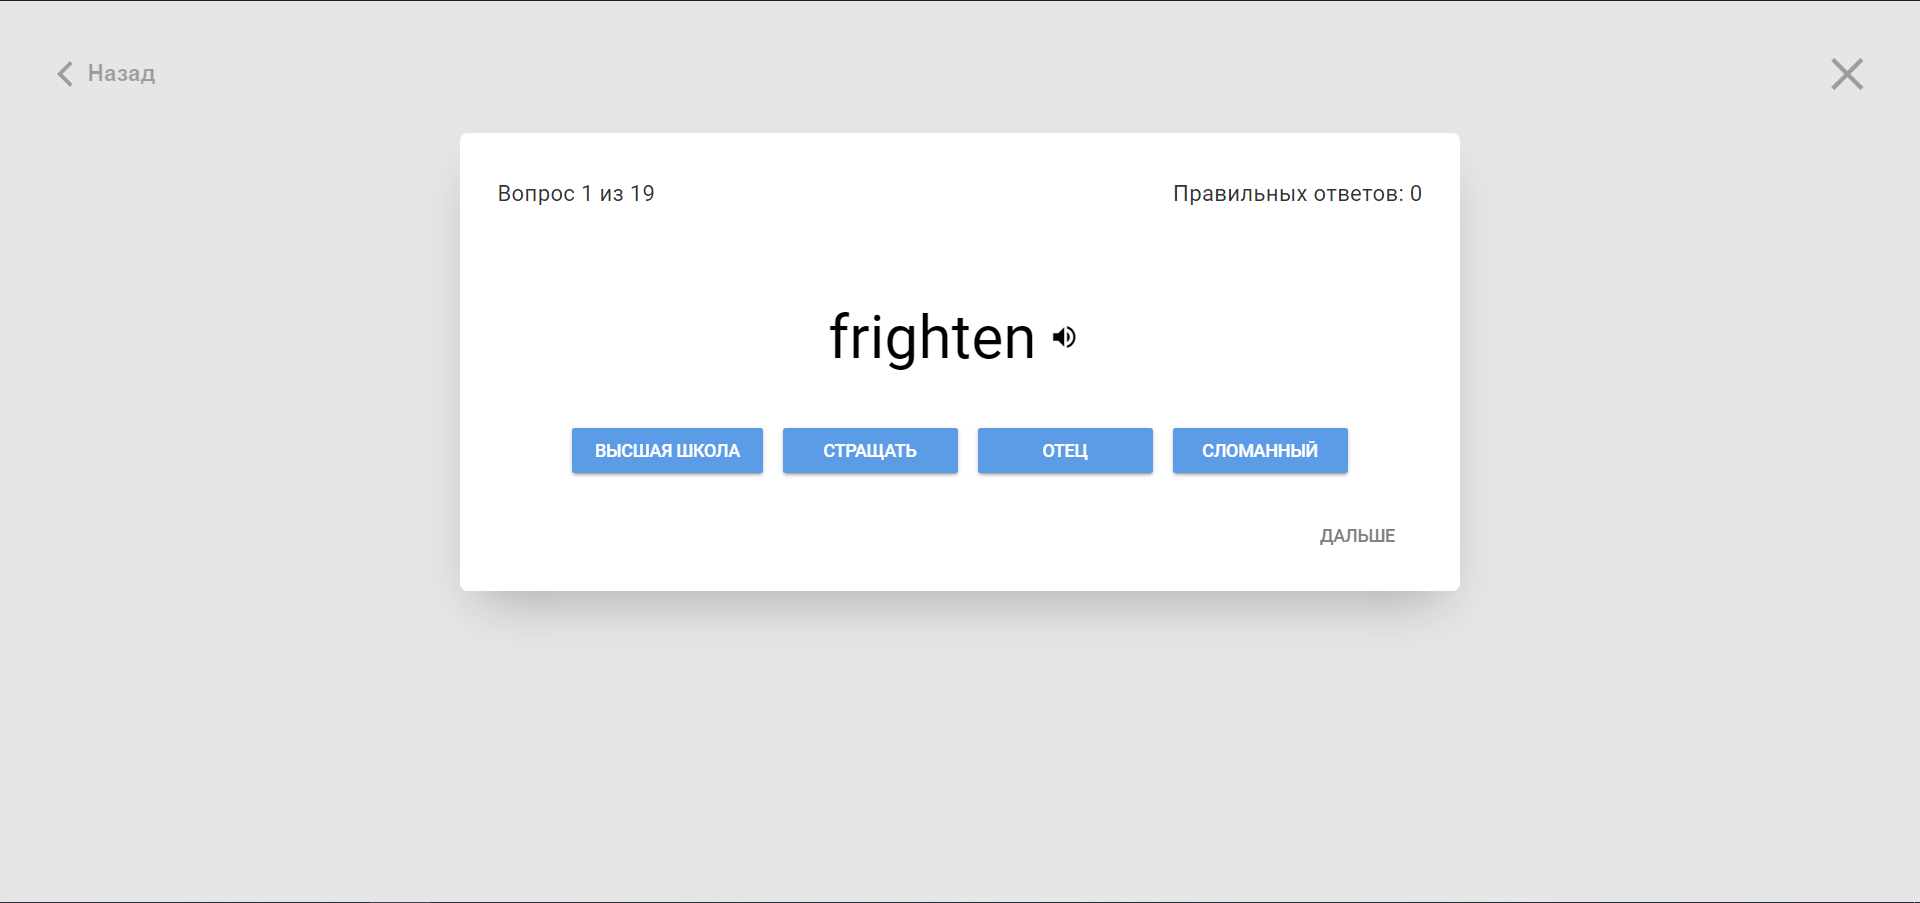
\includegraphics[width=\textwidth]{figures/trainer}
	\caption{Страница с тренажером для изучения слов}
	\label{fig:trainer}
\end{figure}

\begin{figure}[h]
	\centering
	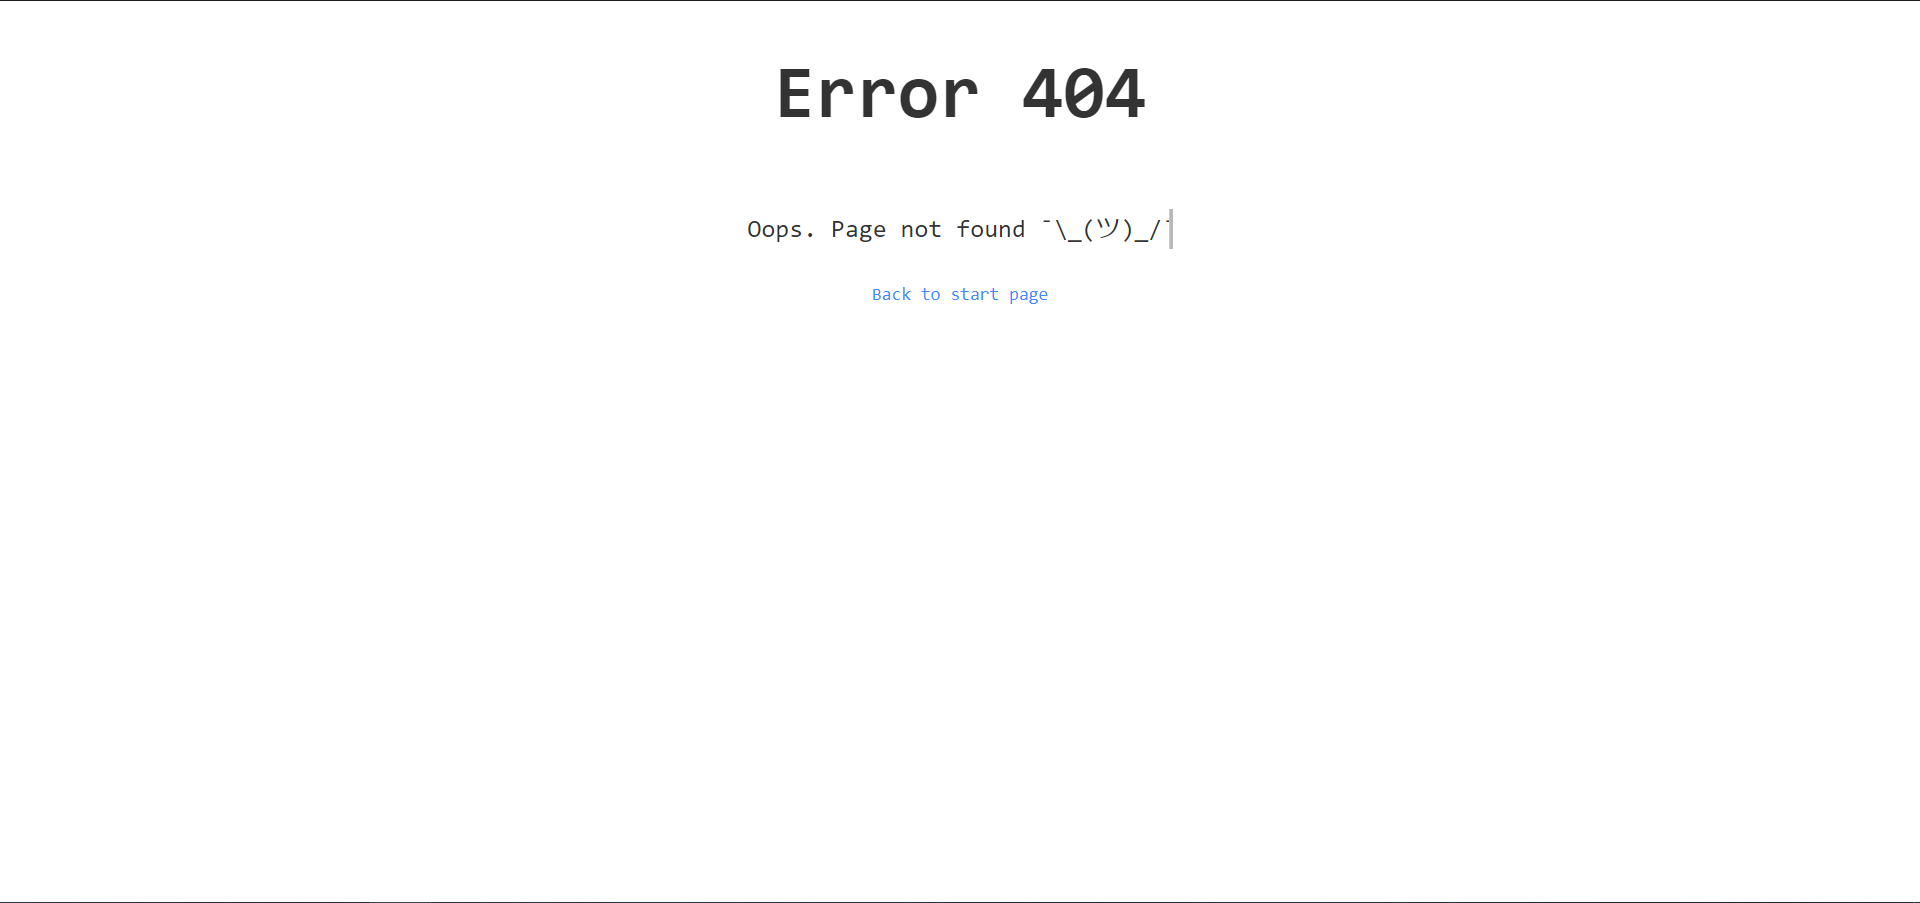
\includegraphics[width=\textwidth]{figures/404}
	\caption{Страница ошибки}
	\label{fig:404}
\end{figure}

%%% Local Variables: 
%%% mode: latex
%%% TeX-master: "rpz"
%%% End: 


\end{document}

%%% Local Variables:
%%% mode: latex
%%% TeX-master: t
%%% End:
